
\documentclass{book}
\usepackage{pervasives}

\title{CMPSCI220 Course Book}

\begin{document}

\maketitle
\tableofcontents

\newlecture

\textbf{Course Description}: Development of individual skills necessary for
designing, implementing, testing and modifying larger programs, including: use
of integrated design environments, design strategies and patterns, testing,
working with large code bases and libraries, code refactoring, and use of
debuggers and tools for version control.

\section{Introduction\classtime{15}}

\emph{CMPSCI220 Programming Methodology} introduces you to all the concepts
above in the context of a modern programming language:
\href{http://www.scala-lang.org/what-is-scala.html}{Scala}.
You could use Scala to write exactly the same kind
of object-oriented code that you've seen in Java. In fact, Scala code and Java
code can seamlessly co-exist and interoperate in the same program; we'll
leverage this feature later in the course. In fact, many of the design patterns
that you will learn in this course will be applicable to Java and Scala.

However, a key reason we're using Scala is to expose you to programming techniques
and language features that are beyond the scope of Java. Most
modern software systems are written in a plethora of languages. In fact, large
systems tend to use several programming languages. Therefore, to succeed in your
computing career, you have to be familiar with several languages and be able to
learn new languages on your own. Programming
languages are constantly invented and abandoned\footnote{\href{http://www.oreillynet.com/pub/a/oreilly/news/languageposter_0504.html}{This poster} is a very incomplete history of the birth and death of programming languages.}
 and it is impossible to predict the next big language that everyone
will use or the language you'll need to learn for your first job.

Scala is a big language with many unique features and we are not going to learn
to use them all. Instead, we are going to focus on ideas that Scala shares with
other modern programming languages. Here are some of the key ideas that we will
cover in this course that go beyond Java:
%
\begin{itemize}

\item \emph{First-class functions} are the cornerstone of \emph{functional programming}.
  They are pervasive in JavaScript, Ruby, Python, Swift, and almost all modern
  languages.

  In fact, even \href{{http://docs.oracle.com/javase/tutorial/java/javaOO/lambdaexpressions.html}}{Java} and
  \href{http://msdn.microsoft.com/en-us/library/dd293608.aspx}{C++} recently
  added support for first-class functions.

\item \emph{Algebraic data types} are available in Apple Swift, Mozilla Rust,
  Microsoft F\#, and several other programming languages. Programming with
  algebraic data types is very different from programming in an object-oriented
  style. We'll cover both styles of programming in this course and develop
  a deep understanding of the tradeoffs.

\item \emph{Type inference} is available in modern typed programming languages,
  such as C\# and Swift, and even in a limited form in
  \href{http://docs.oracle.com/javase/tutorial/java/generics/genTypeInference.html}{Java}.
  As the name suggests, in a language with type inference, the compiler can
  often ``infer'' or fill-in types that you omit. So, your programs become shorter, but
  retain all the advantages of type checking.

\end{itemize}

The main themes of the course are not language-specific. We will emphasize
the following broad ideas that are applicable to all software development:
%
\begin{itemize}

\item \emph{Testing} is critical for building reliable software. You will learn how
  to test complex functions and make effective use of testing tools and frameworks.
  Every programming problem you solve in this course will have to be tested. We
  expect you to write good tests yourself. The quality of your tests will be a
  significant portion of your grade on every assignment.

\item \emph{Design patterns} are recipes for solving typical programming
  problems. This course will emphasize object-oriented and functional
  design patterns. We will focus on design patterns that are applicable to
  a variety of programming languages, and not Scala-specific design patterns.

\item \emph{Refactoring} is a key concept that we emphasize throughout the
  course. As we introduce new ideas, we will systematically refactor our old
  code to exploit them.

\item \emph{Debugging} is a necessary skill because even small programs often
  have bugs.

\item \emph{Command-line tools} such as compilers and build tools lie under the
  hood of sophisticated IDEs such as Eclipse. Learning to use the command-line
  will make you a better IDE user. Moreover, since many new languages lack good
  IDEs, we will emphasize the use of command-line tools in this course.

\item \emph{Version control} software is critical for collaborative software
  development and used by all professional programmers. Although you will be
  programming alone in the course, version control will still help you organize
  your programming and save you a lot of time if you accidentally delete or
  break your code.

\item \emph{Using libraries} is critical for writing software that gets real
  work done. Initially, you'll use libraries that were developed specifically
  for this course, but you will eventually learn to discover and use
  libraries from the Web.

\end{itemize}

The overarching goal of this course is to make you a better programmer,
and an important part of that is to get familiar with programming terminology
and culture. Unfortunately, there is a lot of misinformation on the Web
about programming, but we will try to point you to sources that are reliable.
Here are two good places to start:
%
\begin{itemize}

  \item \href{http://paulgraham.com/articles.html}{Paul Graham's Essays}.
  The earlier essays are particularly pertinent, E.g.,
  \href{http://paulgraham.com/avg.html}{Beating the Averages} and
  \href{http://paulgraham.com/popular.html}{Being Popular}.

  \item \href{http://www.joelonsoftware.com}{Joel Spolsky's blog}. E.g.,
  \href{http://www.joelonsoftware.com/articles/CollegeAdvice.html}
  {Advice for Computer Science College Students}
  and \href{http://www.joelonsoftware.com/articles/ResumeRead.html}
  {Getting Your Resume Read}.

\end{itemize}

Finally, \href{http://xkcd.com}{XKCD} comics often make obscure programming
references and this course will help you decipher some of them.

\section{The Command-Line\classtime{5}}

The \emph{Linux command-line}\footnote{The command-line is also known as a
\emph{terminal} or \emph{shell}.} is  a critical part of this course. If you're
using the course virtual-machine, you should use the program \textbf{LXTerminal}
to start the command-line.

Unless you're already familiar with the Linux command-line, you must read
\href{http://learncodethehardway.org/cli/book/cli-crash-course.html}{Zed Shaw's Command Line Crash Course},
up to and including the chapter ``Removing a File (rm)''. Zed likes to swear at
his own readers, so we'd like to apologize in advance on his behalf. The rest
of these lecture notes assume that you are familiar with the command-line.

\begin{instructor}
\begin{itemize}

\item Introduce the course VM.

\item  Introduce the command line (\verb|mkdir|, \verb|cd|, and, \verb|ls|).
\end{itemize}

\end{instructor}

\section{\sbt{} and the Scala REPL\classtime{5}}

\sbt{} is the Swiss Army Knife of Scala programming. It is a command-line tool
that can be use to run Scala programs, compile them, test them, package them
deployment, publish them to the Web, and more. Like many modern programming
languages, \sbt{} has a \emph{REPL} (read-eval-print loop), which you can use to
type in and run one-line programs immediately, without the bother of creating
files, etc.

To start the Scala REPL, open a terminal (LXTerminal on the course VM),
type in \verb|sbt console| and press enter. Your screen will look like this:
%
\begin{console}
student@vm:~$ sbt console
[info] Loading global plugins from /Users/arjun/.sbt/0.13/plugins
[info] Set current project to del (in build file:/Users/arjun/scratch/del/)
[info] Updating {file:/Users/arjun/}arjun...
[info] Resolving org.fusesource.jansi#jansi;1.4 ...
[info] Done updating.
[info] Starting scala interpreter...
[info]
Welcome to Scala version 2.11.7 (Java HotSpot(TM) 64-Bit Server VM, Java 1.8.0_60).
Type in expressions to have them evaluated.
Type :help for more information.

scala>
\end{console}

The \verb|scala>| prompt indicates that you can type in Scala expressions to evaluate.

\section{Scala Basics\classtime{15}}

\subsection{Simple Expressions and Names}

Arithmetic in Scala is very similar to arithmetic in Java:

\begin{console}
scala> 19 * 17
res0: Int = 323
\end{console}

Strings in Scala will also look familiar:

\begin{console}
scala> "Hello, " + "world"
res1: String = Hello, world
\end{console}

Boolean expressions will be familiar too:

\begin{console}
scala> true && false
res2: Boolean = false
\end{console}

Let's examine the last interaction more closely. When you type \scalainline{true && false},
Scala prints three things:
%
\begin{itemize}
\item An automatically-generated \emph{name} (\scalainline{res2}),
\item The \emph{type} of the expression (\scalainline{Boolean}), and
\item The \emph{value} of the expression (\scalainline{false}).
\end{itemize}

On the Scala REPL, you can use the generated name as a variable. But, you're
better off picking meaningful names yourself using \scalainline{val}:

\begin{console}
scala> val mersenne = 524287
mersenne : Int = 524287
scala> val courseName = "Programming Methodology"
courseName : String = Programming Methodology
\end{console}

\subsection{Type Inference}

You'll find that Scala programs are significantly shorter than their Java
counterparts. A key feature of Scala that lets you write less code is \emph{type
inference}. Notice in the variable definitions above, you did not have to write
any types. Instead, Scala \emph{inferred} them for you. This feature is very helpful
in larger programs, where types can become complex.

Type inference is not magic; later in the course, you'll learn more about how it
works and when it doesn't. For now, here's a rule of thumb: Scala can infer the
type of variable named with \verb|val|. But, Scala \emph{cannot} infer the type of
function parameters.

\subsection{Functions}

Here is a very simple Scala function:

\begin{console}
scala> def double(n: Int): Int = n + n
double: (n: Int)Int
\end{console}

This code defines a function called \scalainline{double}, which takes an argument called
\scalainline{n} of type \scalainline{Int} and returns a value of type \scalainline{Int}. We can apply the
function as follows:

\begin{console}
scala> double(10)
res3: Int = 20
\end{console}

The following function takes two arguments, \scalainline{x} and \scalainline{y} and calculates the
distance from the point \scalainline{(x,y)} to the origin:

\begin{console}
scala> def dist(x: Double, y: Double): Double = math.sqrt(x * x + y * y)
dist: (x: Double, y: Double)Double

scala> dist(3.0, 4.0)
res4: Double = 5.0
\end{console}

Notice that unlike variable definitions, we need \emph{type annotations}
on function parameters and result types.

If your function actually fits on a line (without scrolling off your window),
you can define them very tersely as shown above. But, many interesting
functions span several lines and need local variables.

\subsection{Blocks and Local Variables}

You can define local variables within a \emph{block}. A block is code delimited by
curly-braces. For example:

\begin{console}
scala> def dist2(x: Double, y: Double): Double = {
  val xSq = x * x
  val ySq = y * y
  math.sqrt(xSq + ySq)
}
\end{console}

\begin{figure}
\scalafile{code/Lecture1fac.scala}

\caption{A Scala module}
\label{lecture1code}
\end{figure}

\section{\sbt{} Project Structure\classtime{5}}

In principle, you can write a full-fleged program line-by-line in the Scala
console. But, it makes a lot more sense to save large programs to files
for a particular project. To do so, we will being by creating a new directory
for your project.

First, exit the Scala console by typing \verb|:quit| and then exit \sbt{}
by typing \verb|exit|. You should return to the command-line:
%
\begin{console}
scala> :quit

[success] Total time: 3 s, completed Jan 13, 2016 8:47:38 PM

sbt> exit
student@vm:~$
\end{console}

At the terminal, let's create a directory for the project:
%
\begin{console}
student@vm:~$ mkdir lecture1
\end{console}
%
Then, let's enter the directory:
\begin{console}
student@vm:~$ cd lecture1
student@vm:~/lecture1$
\end{console}
Notice that the name of the directory is displayed on the command-line.

Your Scala projects will have two kinds of files: test cases and your implementation.
\sbt{} requires you to organize your files into the following directory
structure:
\dirtree{%
.1 ~/lecture1.
.2 src.
.3 main.
.4 scala\DTcomment{Implementation goes here}.
.3 main.
.4 scala\DTcomment{Tests goes here}.
}

You can create these directories by running the following commands:
\begin{console}
student@vm:~/lecture1$ mkdir src
student@vm:~/lecture1$ mkdir src/main
student@vm:~/lecture1$ mkdir src/main/scala
student@vm:~/lecture1$ mkdir src/test
student@vm:~/lecture1$ mkdir src/test/scala
\end{console}

We will now see how to save Scala code to files. Using a text editor
(e.g., Sublime Text), create a file called \verb|Lecture1.scala| in the
\verb|src/main/scala| directory, with the contents shown in \cref{lecture1code}.
The code creates an object with a single function to calculate factorials.

\begin{instructor}
Scala wart: Do not \verb|extend App| because it can't be evaluated in console.
\end{instructor}

When you write functions in a Scala file, you \emph{have} to place it in
an object. You cannot just write \scalainline{def fac ...} without an enclosing
object. This is a peculiarity of Scala that we will explain later in the course.
In this example, the name of the object is ``Lecture1'', but it can be anything
you like.

Now that we've saved this function to a file, we can use it from the console:
%
\begin{console}
sbt> console
scala> import Lecture1._
scala> fac(10)
\end{console}

\begin{figure}
\begin{scalacode}
// src/main/scala/Lecture1Tests.scala
import Lecture1._

class Lecture1Tests extends org.scalatest.FunSuite {

  test("fac -- base case") {
    assert(fac(0) == 1)
  }

  test("fac -- inductive case") {
    assert(fac(5) == 120)
  }

}
\end{scalacode}
\caption{Unit tests for the code in \cref{lecture1code}}
\label{lecture1tests}
\end{figure}

\section{Testing\classtime{5}}

The \sbt{} console is a convenient way to experiment with new code or write
a ``one off' functionn. However, you must write \emph{unit tests} to test
any actual code you write. \Cref{lecture1tests} shows an example of
unit tests that use the \emph{ScalaTest} library. The code is quite self-explanatory:
each test suite is a class that extends \scalainline{org.scalatest.FunSuite}.
The body of the class has several test blocks, as shown in the figure.

\begin{instructor}

\begin{itemize}

\item Propose a new function to write. Write the test-cases first, then
the implementation and re-run \verb|sbt test|.

\item Recap the development methodology: first write tests cases, then
write the implementation, and re-test continuously. Show continuous
testing with \verb|~test|.

\end{itemize}


\end{instructor}

\section{Building and Pattern-Matching on Lists\classtime{25}}


In this section, we will show how to write simple list-processing functions. We
will cover basic \emph{functional programming} and introduce \emph{pattern
matching}.

\subsection{Constructing Lists}

The simplest list is the empty list, which is written in Scala as
%
\begin{scalacode}
Nil
\end{scalacode}
%
Given the empty list, we can construct larger lists using the \scalainline{::}
operator (which is pronounced \emph{cons}). Here is a simple example that
constructs a one-element list:
%
\begin{scalacode}
50 :: Nil
\end{scalacode}
Given a one-element list, we can build a two-element list by using the
\scalainline{::} operator again:
%
\begin{scalacode}
100 :: (50 :: Nil)
\end{scalacode}
%
We can use \scalainline{::} again to build a three-element list:
%
\begin{scalacode}
200 :: (100 :: (50 :: Nil))
\end{scalacode}
%
In an expression \scalainline{x :: y},
\scalainline{x} is known as the \emph{head} of the list and \scalainline{y} is
known as the \emph{tail}. Note that the tail of a list is always a list itself,
(though it may be the empty list \scalainline{Nil}).

For example, consider the list below:
\begin{scalacode}
val letters = "a" :: ("b" :: :: Nil)
\end{scalacode}
%
\begin{itemize}

  \item The head of \scalainline{letters} is \scalainline{"a"}.

  \item The tail of \scalainline{letters} is \scalainline{"b" :: Nil}.

  \item The head of the tail of \scalainline{letters} is \scalainline{"b"}.

  \item The tail of the tail of \scalainline{letters} is \scalainline{Nil}.

  \item \scalainline{Nil} does not have a head or a tail.

\end{itemize}

In our examples so far, we've used parenthesis to make the head and tail clear.
However, you can simply write \scalainline{"a" :: "b" :: "c" :: Nil}. Intuitively,
everything to the right of a \scalainline{::} is the tail. If you get confused
up, write the parenthesis explicitly.

It is usually easier to write lists in the following way:
%
\begin{itemize}

  \item \scalainline{List("a", "b", "c")} is equivalent to
  \scalainline{"a" :: ("b" :: ("c" :: Nil))}.

  \item \scalainline{List()} is equivalent to \scalainline{Nil}.

\end{itemize}
%
However, it is important to understand that this is just a convenient notation.
Under the hood, Scala transforms these expressions to use \scalainline{::}
and \scalainline{Nil}, as we described above.

\paragraph{Lists and Type Inference}

You should try to type out the expressions above into the \sbt{} console.
For example:
%
\begin{console}
scala> val lst = 1 :: 2 :: 3 :: Nil
lst: List[Int] = List(1, 2, 3)
\end{console}
%
As you can see, Scala prints lists using the shorthand notation,
even if you explicitly use \scalainline{::} and \scalainline{Nil}.
More significantly, Scala has inferred that the type of the list
is \scalainline{List[Int]}. There was no need to explicitly state that
is is the case.

Here is another example, where Scala infers that the type of a list is
\scalainline{List[String]}:
%
\begin{console}
scala> val lst = List("a", "b", "c")
lst: List[String] = List("a", "b", "c")
\end{console}

Type inference is very convenient and spares you from having to explicitly
specify the type of the element. However, type inference is not magic
and can behave in unexpected ways. For example, in the interaction
below, Scala infers that the type of the list is \scalainline{List[Any]}:
%
\begin{console}
scala> val lst = List("a", 10, "c")
lst: List[Any] = List("a", 10, "c")
\end{console}
Although this is technically true, if you write this code, it is more
likely that you made a mistake and intended to actually create a list of
strings. If you're ever unsure, you can write the type explicitly, which
would signal a type error in this case:
\begin{console}
scala> val lst = List[String]("a", 10, "c")
<console>:10: error: type mismatch;
 found   : Int(10)
 required: String
       val lst = List[String]("a", 10, "c")
                                   ^
\end{console}

\begin{figure}

\begin{subfigure}[b]{0.45\textwidth}
\begin{scalacode}
def countDown(n: Int): List[Int] = {
  if (n == 0) {
    Nil
  }
  else {
    n :: countDown(n - 1)
  }
}
\end{scalacode}
\caption{}
\label{countDown}
\end{subfigure}
\hskip 2em
\begin{subfigure}[b]{0.45\textwidth}
\begin{scalacode}
def fromTo(lo: Int, hi: Int): List[Int] = {
  if (lo == hi) {
    lo :: Nil
  }
  else {
    lo :: fromTo(lo + 1, hi)
  }
}
\end{scalacode}
\caption{}
\label{fromTo}
\end{subfigure}

\caption{Functions that produce lists.}
\label{listcons}
\end{figure}

\paragraph{Functions that produce lists}

Now that we've seen how to construct lists explicitly, it is straightforward
to write functions that produce lists. \Cref{listcons} shows some simple
recursive functions that construct new lists.

\begin{figure}
\begin{subfigure}[b]{0.45\textwidth}
\begin{scalacode}
def product(lst: List[Int]): Int = lst match {
  case Nil => 1
  case n :: rest => n * product(rest)
}
\end{scalacode}
\caption{Calculate the product of a list of numbers.}
\end{subfigure}
\hskip 2em
\begin{subfigure}[b]{0.45\textwidth}
\begin{scalacode}
def repeatTwice(lst: List[Int]): List[Int] = lst match {
  case Nil => Nil
  case n :: rest => n :: n :: repeatTwice(rest)
}
\end{scalacode}
\caption{Repeats every element of a list twice.}
\end{subfigure}

\caption{Two simple functions that consume lists.}
\label{listconsumers}
\end{figure}


\subsection{Pattern Matching}

Now that we've seen how to write functions that produce lists, we'll
learn how to write functions that consume lists as arguments. We'll
start by writing a simple function to calculate the sum of a list of numbers.
Here are some examples of of \scalainline{sum} being used:
%
\begin{scalacode}
assert(sum(20 :: 30 :: Nil) == 50)
assert(sum(1 :: 2 :: 3 :: Nil) == 6)
\end{scalacode}

Intuitively, to calculate \scalainline{sum(1 :: 2 :: 3 :: Nil)}, we can
can recursively calculate the sum of the tail and add that value to the
head:
\begin{scalacode}
   sum(1 :: 2 :: 3 :: Nil)
== 1 + sum(2 :: 3 :: Nil)
== 1 + (2 + sum(3 :: Nil))
== 1 + (2 + (3 + sum(Nil)))
\end{scalacode}
%
The last line shows an important special case. Since the empty list
doesn't have a head or a tail, we need to treat it differently. We'll say
that \scalainline{sum(Nil)} is \scalainline{0}.

We can write \scalainline{sum} by using a powerful feature of
Scala called \emph{pattern matching}.
%
\begin{scalacode}
def sum(lst: List[Int]): Int = {
  lst match {
    case Nil => 0
    case h :: t => h + sum(t)
  }
}
\end{scalacode}
%
This code makes it clear that the function is inspecting \scalainline{lst}
and considering two \emph{cases}. When \scalainline{lst} is \scalainline{Nil},
it produces \scalainline{0} and when \lstinline{lst} is constructed with
the \scalainline{::} operator, the function recurs on the tail and ands
that result to the head. In this code,
\scalainline{Nil} and \scalainline{h :: t} are called \emph{patterns}.

\Cref{listconsumers} shows two more list-consuming functions that
use pattern-matching. Notice that in \scalainline{::} cases, these functions
use different variable names for the head and the tail. A pattern can use
any variable to refer to the value of the head or the tail.

\begin{figure}
\begin{subfigure}[b]{0.45\textwidth}
\begin{scalacode}
def countOnes(lst: List[Int]): Int = lst match {
  case Nil => 0
  case n :: rest => {
    if (n == 1) {
      1 + countOnes(rest)
    }
    else {
      countOnes(rest)
    }
  }
}
\end{scalacode}
\caption{Counting ones using an if-expression.}
\label{countonescomplex}
\end{subfigure}
\hskip 2em
\begin{subfigure}[b]{0.45\textwidth}
\begin{scalacode}
def countOnes(lst: List[Int]): Int = lst match {
  case Nil => 0
  case 1 :: rest => 1 + countOnes(rest)
  case n :: rest => countOnes(rest)

}
\end{scalacode}
\caption{Counting ones using a composite pattern.}
\label{countonessimple}
\end{subfigure}

\caption{Pattern matching can make complex conditionals clearer.}
\end{figure}

\paragraph{Complex Patterns}
%
Pattern-matching is extremely powerful and can be used to express
complex conditionals. For example, \cref{countonescomplex} is a function
that counts the number of \scalainline{1}s that occur in a list: it uses
pattern matching as introduced above and then an if-expression to
check if the head of the list is \scalainline{1}.

\Cref{countonessimple}
is the same function, rewritten to use pattern matching. This version is shorter
and makes it clear that there are three cases. To do so, we exploit the fact
that patterns can match \emph{almost} any value, including numbers,
strings, lists, and user-defined data structures too (which we will see
in a later class).

\paragraph{Exhaustivity and Reachability Checking}
%
Here is another function that uses pattern matching to count the number
of tens in a list:
%
\begin{scalacode}
def countTens(lst: List[Int]): Int = lst match {
  case 10 :: rest => 1 + countTens(rest)
  case n :: rest => countTens(rest)
}
\end{scalacode}

However, this function had a bug. Do you see it? If you type this into
a console, Scala prints the following:
%
\begin{console}
<console>:10: warning: match may not be exhaustive.
It would fail on the following input: Nil
       def countTens(lst: List[Int]): Int = lst match {
                                            ^
\end{console}
%
Scala has detected that we forgot to write a case for \scalainline{Nil}.
Scala ensures that your patterns are \emph{exhaustive}. Here is another
buggy version of the function:
%
\begin{scalacode}
def countTens(lst: List[Int]): Int = lst match {
  case n :: rest => 1 + countTens(rest)
  case n :: rest => countTens(rest)
  case Nil => 0
}
\end{scalacode}
%
In this version, we wrote the patterns incorrectly, so the first and second
patterns are identical. Scala reports the following error:
\begin{scalacode}
<console>:13: warning: unreachable code
         case n :: rest => countTens(rest)
\end{scalacode}
%
Scala ensures that all cases are \emph{reachable}.

This automatic exhaustivity and reachability checking makes programs that
use pattern-matching much more robust than programs that use complicated,
nested if-statements. Pattern matching is a very powerful tool that you can
exploit to make your programs more robust. We will emphasize pattern-matching
over conditionals in this course.

\newhw{Introduction to Scala}

\due{Thursday, Jan 28}

This assignment has several ``finger exercises'' that introduce you
to functional programming in Scala.

\section{Setup}

Before you start programming, you need to complete a few preliminary steps.

\begin{enumerate}

\item Download and start the course virtual machine. You will need it for all
the assignments in this class.

\item Using the command-line, create a directory for your assignment (e.g., the
  \verb|hw1| directory). Within this directory, create the directories
  \verb|src/main/scala| and \verb|src/test/scala|. For example, you could use
  the following commands:
  %
  \begin{console}
  mkdir hw1
  cd hw1
  mkdir src
  mkdir src/main
  mkdir src/main/scala
  mkdir src/test
  mkdir src/test/scala
  \end{console}

   \item Using a text editor, create the file \verb|src/main/scala/Lecture1.scala|
   with the following contents:
   %
   \scalafile{../hw/lists/template/src/main/scala/Lecture1.scala}

   \item Using a text editor, create the file \verb|src/test/scala/TestSuite.scala|
   with the following contents:
   %
   \scalafile{../hw/lists/template/src/test/scala/TestSuite.scala}

  \item From the command-line, start \sbt{} and run the test suite. You should
  see output that looks like this:

  \lstinputlisting[language=console]{../hw/lists/template/test-output.txt}

  \noindent \emph{There should be no errors or warnings printed.}

\end{enumerate}

\section{Exercises}

For this assignment, you'll be writing several list-processing
functions. You must place these within the \verb|Lecture1| object that
you created above. You must write tests cases, within the \verb|TestSuite|
class that you created above.

\begin{enumerate}

  \item Write a function called \scalainline{sumDouble} that consumes a
  \scalainline{List[Int]} and produces an \scalainline{Int}. The produced
  value should be double the sum of the list of integers.

  \item Write a function called \scalainline{removeZeroes} that consumes a
  \scalainline{List[Int]} and produces a \scalainline{List[Int]}.
  The produced list should be the same as the input list, but with all zeroes
  removed. The function must not change the order of elements.

  \item Write a function called \scalainline{countEvens} that consumes a
  \scalainline{List[Int]} and produces an \scalainline{Int} that represents
  that number of even numbers in the input list.

  \item Write a function called \scalainline{removeAlternating} that consumes a
  \scalainline{List[String]} and produces a \scalainline{List[String]} that
  has every other element in the input list.

  The first element of the input list must be in the output list.
  For example:
  \begin{scalacode}
  assert(removeAlternating(List("A", "B")) == List("A"))
  assert(removeAlternating(List("A", "B")) != List("B"))
  \end{scalacode}

  The function must not change the order of elments.

  \item Write a function called \scalainline{isAscending} that consumes a
  \scalainline{List[Int]} and produces a \scalainline{Boolean} that is
  \scalainline{true} if the numbers in the input list are in ascending order.
  Note that the input may have repeated numbers.

  \item Write a function called \scalainline{addSub} that consumes a
  \scalainline{List[Int]} and produces an \scalainline{Int}. The
  function should add all the elements in even position and subtract all the
  elements in odd position.

  Note that the first element of a list is considered
  ``zeroth'' element, thus it is in even position.
  For example, \scalainline{addSub(List(10, 20, 30, 40))} should be
  \scalainline{10 - 20 + 30 - 40}.

  \item Write a function called \scalainline{alternate} that consumes \emph{two}
  \scalainline{List[Int]} arguments and produces a \scalainline{List[Int]}.
  The elements of the resulting list should alternate between the elements of
  the arguments. You may assume that the two arguments have the same
  length.

  For example:

  \begin{scalacode}
  assert(alternate(List(1, 3, 5), List(2, 4, 6)) == List(1, 2, 3, 4, 5, 6))
  \end{scalacode}

  \item Write a function called \scalainline{fromTo} that takes
  two \scalainline{Int}s as arguments and produces a \scalainline{List[Int]}.
  The value of \scalainline{fromTo(x, y)} should be the list of consecutive
  integers that start from and include $x$, going up to and excluding $y$.
  You may assume that $x < y$.

  For example:
  \begin{scalacode}
  assert(fromTo(9, 13) == List(9, 10, 11, 12))
  \end{scalacode}

  \item Write the following function:

  \begin{scalacode}
  def insertOrdered(n: Int, lst: List[Int]): List[Int]
  \end{scalacode}

  Assuming that \scalainline{lst} is in ascending order,
  \scalainline{insertOrdered} should produce a list that is the same as
  the input, but with $n$ inserted such that the order is preserved.
  For example, \scalainline{insertOrdered(5, List(1, 3, 7, 9))} should be
  \scalainline{List(1, 3, 5, 7, 9)}.

  You should assume that \scalainline{lst} is in ascending order. Your function
   may produce any result or even throw an exception if it is not.

   \item Write the following function:

   \begin{scalacode}
   def sort(lst: List[Int]): List[Int]
   \end{scalacode}

   The result should be the sorted input list.

\end{enumerate}

\section{Hand In}

From \sbt{}, run the command \verb|submit|. The command will create
a file called \verb|submission.tar.gz| in your assignment directory.
Submit this file using Moodle.

For example, if the command runs successfully, you will see output similar
to this:
%
\begin{console}
Created submission.tar.gz. Upload this file to Moodle.
[success] Total time: 0 s, completed Jan 17, 2016 12:55:55 PM
\end{console}

\textbf{Note:}  The command will not allow you to submit code that does not
compile. If your code doesn't compile, you will receive no credit for the
assignment.

\newlecture

\begin{instructor}

\section{Lecture 1 Recap\classtime{15}}

\begin{itemize}

  \item Slowly talk through the command-line commands involved in creating,
  changing to it, and starting \sbt{}.

  \item Create a file with a simple list-processing function. E.g., the
  \scalainline{incrList} function below.

  \item Create a test-suite for the function and run it using \sbt{}.


\end{itemize}

\end{instructor}

\begin{figure}
\begin{scalacode}
def incrList(lst: List[Int]): List[Int] = lst match {
  case Nil => Nil
  case head :: tail => (head + 1) :: incrList(tail)
}
\end{scalacode}

\caption{A function that increments all numbers in a list.}
\label{incrlist}
\end{figure}

\section{Immutability \classtime{10}}

\begin{instructor}
This really belongs in the previous lecture, but wasn't emphasized.
There was extra time in the first lecture, so this can easily be
placed there.
\end{instructor}

Consider the function \scalainline{incrList} in \cref{incrlist}, which
increments all numbers in a list. We want to emphasize that \scalainline{incrList}
\emph{produces a new list} and leaves the original list unchanged.

You can observe this behavior in the Scala console:
%
\begin{console}
scala> val original = List(10, 20, 30)
original: List[Int] = List(10, 20, 30)

scala> val result = incrList(original)
result: List[Int] = List(11, 21, 31)

scala> original
res0: List[Int] = List(10, 20, 30)

scala> result
res1: List[Int] = List(11, 21, 31)
\end{console}

At no point did we change or \emph{mutate} the original list. In fact, lists in
Scala are \emph{immutable} data structures. There is no way to update their
head or tail. Programming with immutable data structures is a key part of
\emph{functional programming}, which we will emphasize in the first half
of this course.

\begin{figure}
\begin{subfigure}[b]{.45\textwidth}
\begin{javacode}
public class Point {

  double x;
  double y;

  public Point(double x, double y) {
    this.x = x;
    this.y = y;
  }

}

Point pt = new Point(1, 2)
\end{javacode}
\caption{A Java class that represents a point.}\label{javapoint}
\end{subfigure}
\quad\vrule\quad
%
\begin{subfigure}[b]{.45\textwidth}
\begin{scalacode}
class Point(x : Double, y : Double)
val pt = new Point(1, 2)
\end{scalacode}
\caption{A Scala class that represents a point.}\label{scalapoint}
\end{subfigure}
\caption{Scala code is usually much shorter and simpler than Java code.}
\end{figure}

\section{Case Classes\classtime{10}}

Scala classes tend to be shorter than their
Java counterparts. For example, \cref{javapoint} shows a \scalainline{Point} class
in Java and \cref{scalapoint} shows the equivalent class in Scala, which
is much shorter!
If we start adding methods, you'll have to write
more code in Scala too. But, simple classes tend to be very short.
But, we are not going to use classes yet. Instead, we are going to use
\emph{case classes}, which are unique to Scala.

If you write \scalainline{case class}---
%
\begin{scalacode}
case class Point(x: Double, y: Double)
\end{scalacode}
---instead of just \scalainline{class}, you get several conveniences.
First, you can create values without writing \scalainline{new}:
%
\begin{scalacode}
val pt = Point(1, 2)
\end{scalacode}
%
Second, case classes have an automatically generated \scalainline{toString}
method that prints the fields:
%
\begin{console}
scala> pt
pt: Point = Point(1.0,2.0)
\end{console}
%
Finally, all fields are public by default, so you can easily write simple
functions, such as this one, without writing getters:
%
\begin{scalacode}
def magnitude(pt: Point) : Double = {
  math.sqrt(pt.x * pt.x + pt.y * pt.y)
}

test("3-4-5 triangles") {
  assert(magnitude(Point(3, 4)) == 5)
}
\end{scalacode}

\section{Sealed Case Classes\classtime{20}}

Imagine you're a new age librarian, tasked with cataloging information on the
Internet. There are many types of information. Here are some significant ones:

\begin{scalacode}
case class Tweet(user: String, number: Long)
case class Xkcd(number: Int)
case class HackerNews(item: Int, points: Int)
\end{scalacode}

Here are some examples:

\begin{scalacode}
// https://twitter.com/PLT_Borat/status/248038616654299136
val tweet = Tweet("PLT_Borat", 248038616654299136L)
// http://xkcd.com/1316/
val comic = Xkcd(1316)
// https://news.ycombinator.com/item?id=8169367
val news = HackerNews(8169367, 305)
\end{scalacode}

Let's write a function called \verb|getURL| that maps these items to their URLs,
which is easy to do with pattern matching.

\begin{scalacode}
def getURL(item: Any): String = item match {
  case Tweet(user, number) => "https://twitter.com/" + user + "/status/" + number
  case Xkcd(number) => "http://xkcd.com/" + number
  case HackerNews(item, _) => "http://news.ycombinator.com/item?id=" + item
  case _ => sys.error("not a library item")
}
\end{scalacode}

This definition is unsatisfactory. \verb|getURL| takes values of \verb|Any|
type. So, it is really easy to get a runtime error:

\begin{console}
scala> getURL("hello")
java.lang.RuntimeException: not a library item
 at scala.sys.package$.error(package.scala:27)
  at cmpsci220.package$$anonfun$1.apply(package.scala:13)
  at cmpsci220.package$$anonfun$1.apply(package.scala:13)
  at .getURL(<console>:38)
  ... 33 elided
\end{console}

To eliminate this kind of error, we need an \verb|Item| type:

\begin{scalacode}
sealed trait Item
case class Tweet(user: String, number: Long) extends Item
case class Xkcd(number: Int) extends Item
case class HackerNews(item: Int, points: Int) extends Item
\end{scalacode}

A \emph{trait} in Scala is like an \emph{interface}. They're also much more
versatile than interfaces, but we'll get into that later.

Now, we can rewrite \verb|getURL|, restricting the argument type:

\begin{scalacode}
def getURL(item: Item): String = item match {
  case Tweet(user, number) => "https://twitter.com/" + user + "/status/" + number
  case Xkcd(number) => "http://xkcd.com/" + number
  case HackerNews(item, _) => "http://news.ycombinator.com/item?id=" + item
}
\end{scalacode}

This time, applying \verb|getURL| to a non-item produces a type error as expected:

\begin{console}
scala> item("hello")
<console>:43: error: type mismatch;
 found   : String("hello")
 required: Item
              getURL("hello")
\end{console}

A really nice feature of \scalainline{match} is that it checks to ensure you've handled all
cases. For example, suppose we forgot to write the HackerNews case. Scala
prints the following error:

\begin{console}
<console>:18: warning: match may not be exhaustive.
It would fail on the following input: HackerNews(_, _)
       def getURL(item: Item): String = item match {
                                        ^
error: No warnings can be incurred under -Xfatal-warnings.
\end{console}

\paragraph{More Pattern Matching}

You can use \scalainline{match} to also match concrete values. For example, here is
variant of getURL that censors a particular tweet from PLT Borat:

\begin{scalacode}
def getURL(item: Item): String = item match {
  case Tweet("PLT_Borat", 301113983723794432L) => "http://disney.com"
  case Tweet(user, number) => "https://twitter.com/" + user + "/status/" + number
  case Xkcd(number) => "http://xkcd.com/" + number
  case HackerNews(item, _) => "http://news.ycombinator.com/item?id=" + item
}
\end{scalacode}

Imagine you'd added the censoring line, but accidentally removed the line
that handles all other Tweets. Again, Scala will catch the error:

\begin{console}
<console>:62: warning: match may not be exhaustive.
It would fail on the following inputs:
  Tweet("PLT_Borat", (x: Long forSome x not in 301113983723794432L)),
  Tweet((x: String forSome x not in "PLT_Borat"), 301113983723794432L),
  Tweet((x: String forSome x not in "PLT_Borat"), _),
  Tweet(_, (x: Long forSome x not in 301113983723794432L))
       def getURL(item: Item): String = item match {
                                        ^
error: No warnings can be incurred under -Xfatal-warnings.
\end{console}

It is a long error message. But, if you read it carefully, you'll see that it is
very precisely describing exactly the cases that are missing.

\section{Binary Search Trees\classtime{20}}

\begin{figure}
\begin{scalacode}
sealed trait SBinTree
case class SNode(lhs: BinTree, key: Int, value: String, rhs: BinTree) extends SBinTree
case class SLeaf() extends SBinTree

def find(k: Int, t: SBinTree): String = t match {
  case SLeaf() => sys.error("not found")
  case SNode(_, key, value, _) if (k == key) => value
  case SNode(lhs, key, _, _) if (k < key) => find(k, lhs)
  case SNode(_, key, _, rhs) => find(k, rhs)
}

def insert(k: Int, v: String, t: SBinTree): SBinTree = t match {
  case SLeaf() => SNode(SLeaf(), k, v, SLeaf())
  case SNode(lhs, key, _, rhs) if (k == key) => SNode(lhs, key, v, rhs)
  case SNode(lhs, key, value, rhs) if (k <= key) =>  SNode(insert(k, v, lhs), key, value, rhs)
  case SNode(lhs, key, value, rhs) => SNode(lhs, key, value, insert(k, v, rhs))
}

def size(t: BinTree): SBinTree = t match {
  case SLeaf() => 1
  case SNode(lhs, k, v, rhs) => size(lhs) + size(rhs) + 1
}
\end{scalacode}

\caption{Binary search trees.}
\label{bintree}
\end{figure}

\Cref{bintree} shows a type definition for binary search trees, where
keys are integers and values are strings (which is why we call them
\scalainline{SBinTree}s). There are two
kinds of binary trees: (1) empty trees, or \scalainline{SLeaf()}s, and (2)
non-empty trees, or \scalainline{SNode(..)}s, which have a left-subtree,
a numeric key, a string value, and a right-subtree.
Given this definition, we can write canonical functions such
as \scalainline{size}, \scalainline{find}, and \scalainline{insert},
as shown in the same figure.
We emphasize that the \scalainline{insert} function does not modify the
original tree, and instead produces a new binary tree with the element added.


\subsection{Testing}

There is a lot of code in \cref{bintree} that needs to be tested and there
are two categories of tests that we can write. First, we should \emph{test all the
cases} of a function. For example, the \scalainline{insert} function has
four cases and the four tests below are chosen to exercise each case:
\begin{scalacode}
test("insert into empty tree") {
  assert(insert(200, "A", SLeaf()) == SNode(SLeaf(), 200, "A", SLeaf()))
}

test("insert into left-subtree") {
  assert(insert(200, "A", SNode(SLeaf(), 500, "B", SLeaf()))
    == SNode(SNode(SLeaf(), 200, "A", SLeaf()), 500, "B", SLeaf()))
}

test("insert into right-subtree") {
  assert(insert(700, "A", SNode(SLeaf(), 500, "B", SLeaf()))
    == SNode(Leaf(), 500, "B", SNode(SLeaf(), 700, "A", SLeaf())))
}

test("insert and replace") {
  assert(insert(200, "A", SNode(SLeaf(), 200, "B", SLeaf()))
    == SNode(SLeaf(), 200, "A", SLeaf()))
}
\end{scalacode}

A robust test suite should exercise \scalainline{insert} on larger examples, but
it is important to understand exactly what each case is doing, which is what the
descriptive string states.

The second kind if test is to \emph{test properties that relate functions
to each other}. There isn't a neat recipe for these kinds of tests. You have
to think hard about what your code is actually doing. But, here
are some properties for binary trees.

\begin{property}
After we insert a key-value into a tree, we should be able to
find it again.
\end{property}

The following tests check that this property holds on examples
where a key-value is inserted on the left, inserted on the right, or replaces
the root:
%
\begin{scalacode}
val t1 = SNode(SLeaf(), 200, "A", SLeaf())

test("find after insert on right") {
  assert(find(500, insert(500, "B", t1)) == "B")
}

test("find after insert on left") {
  assert(find(100, insert(100, "B", t1)) == "B")
}

test("find after insert replaces") {
  assert(find(200, insert(200, "B", t1)) == "B")
}
\end{scalacode}

\begin{property}
Inserting a key-value into a binary tree produces a tree with size one
greater than the original tree.
\end{property}

The following tests check that this property holds for the three
cases of \scalainline{insert}:
%
\begin{scalacode}
val t1 = SNode(SLeaf(), 200, "A", SLeaf())

test("insert increases size (rhs)")
  assert(size(insert(500, "B", t1) == size(t1) + 1)
}

test("insert increases size (lhs)") {
  assert(size(insert(100, "B", t1) == size(t1) + 1)
}

test("insert increases size (replacement)") {
  assert(size(insert(200, "B", t1) == size(t1) + 1)
}
\end{scalacode}

Unfortunately, the third test case fails because the property is wrong.
When \scalainline{insert} replaces a value in the tree, the size of the tree
does not change. Here is a revised version of this property that accounts
for this corner-case:

\begin{property}
Inserting a key-value into a binary tree either (1) produces a tree with
size one greater than the original tree or (2) the size of the produced
tree is the same and the key was present in the original tree.
\end{property}

We can write a function to test this property for any given $k$, $v$, and $t$
and use it to write our tests compactly:

\begin{scalacode}
def check(k: Int, v: String, t: SBinTree): Boolean = {
  if (size(insert(k, v, t)) == size(t) + 1) {
    true
  }
  else {
    try {
      val r = find(k, t)
      true
    }
    catch {
      case exn:Exception => false
    }
  }
}

val t1 = SNode(SLeaf(), 200, "A", SLeaf())

test("insert increases size (rhs)")
  assert(check(500, "B", t1))
}

test("insert increases size (lhs)") {
  assert(check(100, "B", t1))
}

test("insert increases size (replacement)") {
  assert(check(200, "B", t1))
}
\end{scalacode}

There are other properties that we can test. For example:
%
\begin{scalacode}
insert(k, v, insert(k, v, t)) == insert(k, v, t)
\end{scalacode}

Moreover, if we write more functions to process binary trees, the number of
interesting properties will keep growing.

\section{Lists\classtime{10}}

Although we've used Scala's builtin lists, we can use case classes to write
very similar types. For example, we can write a type for lists of integers
as follows:
%
\begin{scalacode}
sealed trait IList
case class INil() extends IList
case class ICons(head: Int, tail: IList) extends IList
\end{scalacode}

The following function adds $n$ to every number in a list:
%
\begin{scalacode}
def add(n: Int, lst: IList): IList = lst match {
  case INil() => INil()
  case ICons(head, tail) => ICons(head + n, add(n, tail))
}
\end{scalacode}

A test suite should test the two cases in the function. Moreover, we can
also test simple properties of this function alone.

For example, for all \scalainline{m}, \scalainline{n}, and \scalainline{lst}:
%
\begin{scalacode}
add(n, add(m, lst)) == add(m + n, lst)
\end{scalacode}

The following function appends two lists together:
%
\begin{scalacode}
def append(lst1: IList, lst2: IList): IList = lst1 match {
  case INil() => lst2
  case ICons(head, tail) => ICons(head, append(tail, lst2))
}
\end{scalacode}

Again, we should test the two cases of this function. But, there are
several other properties that we can test. For example, if we append
three lists together, the order in which we apply the function
does not matter:
%
\begin{scalacode}
append(lst1, append(lst2, lst3)) == append(append(lst1, lst2), lst3)
\end{scalacode}
i.e., \scalainline{append} is \emph{associative}.

Here is another property of \scalainline{append}:
\begin{scalacode}
append(lst, INil()) == lst
\end{scalacode}
%
Notice that this is \emph{not} a case of \scalainline{append}: the function
pattern-matches on the first argument. This property shows that both cases
of \scalainline{append} behave in a similar way when the second argument is
\scalainline{INil()}.

Finally, we can write properties that relate the \scalainline{add} and
\scalainline{append} functions:
%
\begin{scalacode}
append(add(n, lst1), add(n, lst2)) == add(n, append(lst1, lst2))
\end{scalacode}

\newdiscussion{Homework 1 Help Session (Jan 27)}

\newlecture

\section{Generics and Type Inference\classtime{15}}

\begin{figure}
\begin{minipage}{0.45\textwidth}
\begin{scalacode}
def ilength(lst : List[Int]): Int = lst match {
  case Nil => 0
  case _ :: tail => 1 + ilength(tail)
}
\end{scalacode}
\subcaption{Length of a list of integers.}
\end{minipage}
\quad\vrule\quad
\begin{minipage}{0.45\textwidth}
\begin{scalacode}
def slength(lst : List[String]): Int = lst match {
  case Nil => 0
  case _ :: tail => 1 + slength(tail)
}
\end{scalacode}
\subcaption{Length of a list of integers.}
\end{minipage}
\caption{Two very similar length functions.}
\label{monolength}
\end{figure}

\Cref{monolength} shows two functions that calculate (1) the length of a list
of integers and (2) the length of a list of strings. These two functions
are almost identical. The only difference between them in the type of
element in the list. We can abstract away the differences by writing
a \emph{generic} length function:
%
\begin{scalacode}
def length[A](lst: List[A]): Int = lst match {
  case Nil => 0
  case _ :: tail => 1 + length(tail)
}
\end{scalacode}

In the code above, \verb|A| is a \emph{type argument}. It truly is an argument
to the function, just like \verb|lst|. i.e., when \scalainline{length} is
invoked, we need to specify \verb|A|:
%
\begin{scalacode}
length[Int](List(1, 2, 3))
length[String](List("A", "B", "C", "D"))
\end{scalacode}
%
However, \verb|A| holds a type instead of a value.

Scala lets you elide type arguments in most cases. So, we could also write:
%
\begin{scalacode}
length(List(1, 2, 3))
length(List("A", "B", "C", "D"))
\end{scalacode}
%
But, it is important to note that under the hood, Scala figures out that we
meant \scalainline{A} to be \scalainline{Int} on the first line and
\scalainline{String} on the second line and inserts the type arguments for us.
In fact, we relied on this in the definition of \scalainline{length}: Scala
expands the recursive call \scalainline{length(tail)} to
\scalainline{length[A](tail)}. Note that Scala isn't just ``guessing'' the
right type. It uses the type of the value-arguments to infer the missing
type argument.

However, Scala's type inference is not perfect. It saves you typing, but don't
expect it to figure out exactly what you mean. It can make mistakes.
For example, if we write \scalainline{List(1, "2", 3)}, Scala infers
that it has type \scalainline{List[Any]}. But, this is almost certainly
not what we meant! We probably meant to construct a list of integers
or strings. If we instead wrote \scalainline{List[Int](1, "2", 3)}, Scala
would have signalled a type error.

\subsection{Generic Data Structures}

\begin{figure}

\begin{minipage}{0.45\textwidth}
\begin{scalacode}
sealed trait IBinTree
case class ILeaf() extends IBinTree
case class INode(
  lhs: IBinTree,
  key: Int,
  value: Int,
  rhs: IBinTree)
  extends IBinTree
\end{scalacode}
\caption{Values are integers.}
\end{minipage}
\quad\vrule\quad
\begin{minipage}{0.45\textwidth}
\begin{scalacode}
sealed trait SBinTree
case class SLeaf() extends IBinTree
case class SNode(
  lhs: SBinTree,
  key: Int,
  value: String,
  rhs: SBinTree)
  extends SBinTree
\end{scalacode}
\caption{Values are strings.}
\end{minipage}
\caption{Two non-generic binary trees.}
\label{monobintrees}
\end{figure}

\Cref{monobintrees}
In the last lecture, we build a data structure that represents binary
search trees with strings for values. We can write a similar data structure
with integer-values, as shown in \cref{monobintrees}. But, this will force
us to redefine the functions we wrote earlier to proceed \scalainline{SBinTree}s.
Instead, we can write a generic type for binary trees where the values have
some unknown type \scalainline{A}:

%
\begin{scalacode}
sealed trait BinTree[A]
case class Leaf[A]() extends BinTree[A]
case class Node[A](lhs: BinTree[A], key: Int, value: A, rhs: BinTree[A]) extends BinTree[A]
\end{scalacode}

Here are some examples of binary trees with values of different types:

\begin{itemize}

\item This binary tree has integer values:
\begin{scalacode}
Node(Leaf(), 10, 500, Leaf())
\end{scalacode}

\item This binary tree has string values:
\begin{scalacode}
Node(Leaf(), 10, "five hundred", Leaf())
\end{scalacode}

\item This binary tree has boolean values:
\begin{scalacode}
Node(Leaf(), 10, true, Leaf())
\end{scalacode}

\end{itemize}

We can easily update the \scalainline{insert}, \scalainline{find}, and \scalainline{size}
functions from the last lecture to work with generic binary trees.

\section{Higher-Order Functions on Lists}


\begin{figure}
\begin{subfigure}[b]{.45\textwidth}
\begin{scalacode}
def incrs(lst: List[Int]): List[Int] =
  lst match {
    case Nil => Nil
    case h :: t => h + 1 :: incrs(t)
  }
\end{scalacode}
\caption{A function that increments all numbers in a list.}
\end{subfigure}
\quad\vrule\quad
\begin{subfigure}[b]{.45\textwidth}
\begin{scalacode}
def lengths(lst: List[String]): List[Int] =
  lst match {
  case Nil => Nil
  case h :: t => h.length :: lengths(t)
}
\end{scalacode}
\caption{A function that calculates the lengths of all strings in a list.}
\end{subfigure}
\quad
\vskip 1em \hrule \vskip 1em
\begin{subfigure}[b]{.45\textwidth}
\begin{scalacode}
def doubles(lst: List[Int]): List[Int] =
  lst match {
    case Nil => Nil
    case h :: t => h * 2 :: doubles(t)
}
\end{scalacode}
\caption{A function that doubles all numbers in a list.}
\end{subfigure}
\quad\vrule\quad
\begin{subfigure}[b]{.45\textwidth}
\begin{scalacode}
def negates(lst: List[Int]): List[Int] =
  lst match {
    case Nil => Nil
    case h :: t => -h :: negates(t)
}
\end{scalacode}
\caption{A function that negates all numbers in a list.}
\end{subfigure}

\caption{Four different functions that transform elements of a list.}
\label{map_motivation}
\end{figure}


\subsection{The Map Function\classtime{15}}

Study the four functions in \cref{map_motivation}. The function \verb|incrs|
adds one to every element in a list of integers, the function \verb|lengths|
calculates the length of every string in a list, the function \verb|doubles|
doubles every number in a list, and the function \verb|negates| negates every
number in a list. Hopefully, you've noticed that these four functions have a lot
of in common. \emph{The only difference between them is the operation that they
perform on the head of the list}.

Here is a variant of \verb|doubles| that makes the operation explicit, by
moving it into a separate function:
%
\begin{scalacode}
def f(n: Int): Int = n * 2

def doubles(lst: List[Int]): List[Int] = lst match {
  case Nil => Nil
  case h :: t => f(h) :: doubles(t)
}
\end{scalacode}

In this version, we're simply applying a function $f$ to $h$, where $f$
is the doubling function. \emph{You should apply the same refactoring to the other
functions}. E.g.,  instead of directly writing \scalainline{head.length}, refactor
the function so that this expression is in a helper function.

Once we've re-written the operation as \scalainline{f(h)}, all three
functions look identical: the only difference is that each refers to a
different function.
Instead of writing three functions that are almost identical, we can
write one function that takes $f$ as an argument:

\begin{scalacode}
def map(f: Int => Int, lst: List[Int]): List[Int] = lst match {
  case Nil => Nil
  case h :: t => f(h) :: map(f, t)
}
\end{scalacode}

With this function, we can make our examples much more succinct:

\begin{scalacode}
def doubles(lst: List[Int]) = {
  def f(n: Int): Int = n * 2
  map(f, lst)
}

def incrs(lst: List[Int]) = {
  def f(n: Int): Int = n + 1
  map(f, lst)
}

def lengths(lst: List[String]) = {
  def f(str: String): Int = str.length
  map(f, lst)
}
\end{scalacode}

Unfortunately, the definition of \scalainline{lengths} above does not
type-check. Scala reports two type errors and they are both very informative:

\begin{console}
<console>:15: error: type mismatch;
 found   : String => Int
 required: Int => Int
         map(f, lst)
             ^
<console>:15: error: type mismatch;
 found   : List[String]
 required: List[Int]
         map(f, lst)
                  ^
\end{console}

The \scalainline{map} function only works of lists of integers. However, if you
look at the definition of \scalainline{map} closely, you'll see that all the
\scalainline{Int}-specific code has been factored out into \scalainline{f}. We
can make the function even more generic by introducing two type-parameters:

\begin{scalacode}
def map[A,B](f: A => B, lst: List[A]): List[B] = lst match {
  case Nil => Nil
  case h :: t => f(h) :: map[A, B](f, t)
}
\end{scalacode}

The type-parameter $A$ is the type of the elements in
\emph{lst} and the type-parameter $B$ is the type elements in the produced list.
In the code above, we've make all the type-arguments explicit. But, as we've
discussed before, we can rely on type-inference to fill them in:

\begin{scalacode}
def map[A,B](f: A => B, lst: List[A]): List[B] = lst match {
  case Nil => Nil
  case h :: t => f(h) :: map(f, t)
}
\end{scalacode}

\subsection{The Filter Function\classtime{10}}

Another common pattern when programming with lists is to select certain elements
that have some property. For example, here is a function that consumes a list,
and produces a new list that only contains the even numbers:

\begin{scalacode}
def filterEven(lst: List[Int]): List[Int] = lst match {
  case Nil => Nil
  case head :: tail =>
    (head % 2 == 0) match {
      case true => head :: filterEven(tail)
      case false => filterEven(tail)
    }
}
\end{scalacode}

This is a very common pattern too. For example, we could write a function to
select the odd numbers or the prime numbers. If we had a list of strings, we
could select all the strings with length 5 or all the strings that represent
English-language words. All these functions have the same shape: they test
the value of \scalainline{head} in some way. If the test succeeds, \scalainline{head} is added in
the output list. But, if the test fails, it is excluded.

Following the same strategy we used to derive \scalainline{map}, we first package
the \scalainline{head}-test into a function:

\begin{scalacode}
def f(n: Int): Boolean = head % 2

def filterEven(lst: List[Int]): List[Int] = lst match {
  case Nil => Nil
  case head :: tail =>
    f(head) match {
      case true => head :: filterEven(tail)
      case false => filterEven(tail)
    }
}
\end{scalacode}

Now that the pattern is clearer, we generalize \scalainline{filterEven} to take \scalainline{f}
as an argument:

\begin{scalacode}
def filter(f: Int => Boolean, lst: List[Int]): List[Int] = lst match {
  case Nil => Nil
  case head :: tail =>
    f(head) match {
      case true => head :: filter(f, tail)
      case false => filter(f, tail)
    }
}

def filterEven(lst: List[Int]): List[Int] = {
  def f(n: Int): Boolean = head % 2
  filter(f, lst)
}
\end{scalacode}

Finally, just as we did for \scalainline{map}, we can generalize the type of \scalainline{filter}
so that it can be applied to \scalainline{List[A]}:

\begin{scalacode}
def filter[A](f: A => Boolean, lst: List[A]): List[A] = lst match {
  case Nil => Nil
  case head :: tail =>
    f(head) match {
      case true => head :: filter(f, tail)
      case false => filter(f, tail)
    }
}
\end{scalacode}

\begin{instructor}
Cannot show find because it relies on Option
\end{instructor}

% \subsection{The Find Function\classtime{10}}

% Another common operation on lists is to find an element. For example,
% the following function finds the first even number in a list:

% \begin{scalacode}
% def findEven(lst: List[Int]): Option[Int] = lst match {
%   case Empty() => None()
%   case Cons(head, tail) => (head % 2 == 0) match {
%     case true => Some(head)
%     case false => findEven(tail)
%   }
% }
% \end{scalacode}

% If we change \scalainline{(head % 2 == 0)} to \scalainline{(head % 2 == 1)}, we'll have the
% \scalainline{findOdd} function. Again, instead of defining two slightly different
% functions, we can write the general \scalainline{find} function:

% \begin{scalacode}
% def find[A](f: A => Boolean, lst: List[A]): Option[A] = lst match {
%   case Empty() => None()
%   case Cons(head, tail) => f(head) match {
%     case true => Some(head)
%     case false => find(f, tail)
%   }
% }
% \end{scalacode}

\subsection{Sorting}

You've written sorting functions that sort lists is ascending or descending
order. But, the following higher-order function can be used to sort any
lists of any type, given an arbitrary ``less than'' operator.

\begin{scalacode}
def insert[A](lessThan: (A, A) => Boolean, x: A, lst: List[A]): List[A] = lst match {
  case Nil => List(x)
  case hd :: tl => {
    if (lessThan(x, hd)) {
      x :: hd :: tl
    }
    else {
      hd :: insert(lessThan, x tl)
    }
  }
}

def sort[A](lessThan: (A, A) => Boolean, lst: List[A]) = lst match {
  case Nil => Nil
  case hd :: tl => insert(lessThan, hd, sort(lessThan, tl))
}

def sortAscending(lst: List[Int]): Int = {
  def f(x: Int, y: Int): Boolean = x < y
  sort(f, lst)
}

def sortDescending(lst: List[Int]): Int = {
  def f(x: Int, y: Int): Boolean = x > y
  sort(f, lst)
}

def sortByLengthAscending(lst: List[String]): Int = {
  def f(x: String, y: String): Boolean = x.length < y.length
  sort(f, lst)
}
\end{scalacode}

\section{Builtin Methods on Lists\classtime{5}}

All the higher-order list-processing functions that we've defined are already
built-in to Scala as methods on lists.

\begin{itemize}

\item
We can map over a list using the \scalainline{map} method:

\begin{scalacode}
def f(n: Int): Int = n + 1

assert(List(10, 20, 30).map(f) == List(11, 21, 22))
\end{scalacode}

\item We can filter a list using the \scalainline{filter} method:

\begin{scalacode}
def f(n: Int): Boolean = n % 2 == 0

assert(List(0, 1, 2, 3, 4, 5).map(f) == List(0, 2, 4))
\end{scalacode}

\item We can sort a list using the \scalainline{sortWith} method:

\begin{scalacode}
def f(x: Int, y: Int): Boolean = x > Y

assert(List(3, 7, 9, 11).sortWith(f) == List(11, 9, 7, 3))
\end{scalacode}

\end{itemize}

There are several other higher-order functions that you can discover from
the documentation or the Scala console.

\newhw{Higher-Order Functions}

In this assignment, you'll write several higher-order functions over lists. You
should place all the functions below within an object called
\scalainline{Homework2}.

\textbf{Restrictions}: You must not use Scala's builtin methods. You
may not use imperative features, such as \scalainline{while} and \scalainline{var}.
Feel free to reuse or modify any code your wrote for the previous assignment.
You should also write any helper functions you think are necessary. You
may also use functions you write for one part of the assignment to solve
another part of the assignment.

\section{Exercises}

\begin{enumerate}

\item
Write the \scalainline{map2} function, which maps over two lists:

\begin{scalacode}
def map2[A,B,C](f: (A, B) => C, lst1: List[A], lst2: List[B]): List[C]

test("map2 with add") {
  def add(x: Int, y: Int): Int = x + y
  assert(map2(add, List(1, 2, 3), List(4, 5, 6)) == List(5, 7, 9))
}
\end{scalacode}

You may assume that \scalainline{lst1} and \scalainline{lst2} have the same
length (i.e., do whatever you think is reasonable).

\item
Scala lets you write \scalainline{(x, y)} to create \emph{tuples}. For example:

\begin{scalacode}
val nameSsn: (String, Int) = ("John Smith", 19970293)
val emailAdmin: (String, Boolean) = ("carberry@cs.umass.edu", true)
val xy: (Double, Double) = (3.0, 4.0)
\end{scalacode}

Tuples are a convenient way to package two related values together, without
having to create a new type to hold them. You can use pattern matching to
extract the components of tuples, or simply write \scalainline{xy._1}
and \scalainline{xy._2} to access the first and second component respectively.

Write the \scalainline{zip} function, which tuples corresponding elements in a list:

\begin{scalacode}
def zip[A,B](lst1: List[A], lst2: List[B]): List[(A, B)]

test("zip test 1") {
  assert(zip(List(1, 2, 3), List(4, 5, 6)) == List((1,4), (2, 5), (3, 6)))
}

test("zip test 2") {
  assert(zip(List("George", "Teddy"), List("Washington", "Roosevelt")) ==
         List(("George", "Washington"), ("Teddy", "Roosevelt")))
}
\end{scalacode}

\item
Write the function \scalainline{flatten}, which flattens a nested list:

\begin{scalacode}
def flatten[A](lst: List[List[A]]): List[A]

test("flatten test") {
  assert(flatten(List(List(1, 2), List(3, 4))) == List(1, 2, 3, 4))
}
\end{scalacode}

\item
Write the \scalainline{flatten3} function, which flattens a triple-nested list:

\begin{scalacode}
def flatten3[A](lst: List[List[List[A]]]): List[A]
\end{scalacode}

\item
Write the \scalainline{buildList} function, which builds a list of the given length. Each
element is determined by applying \scalainline{f} to the index of the element:

\begin{scalacode}
def buildList[A](length: Int, f: Int => A): List[A]

test("buildList test") {
  def f(x: Int) = x
  assert(buildList(10, f) == List(0, 1, 2, 3, 4, 5, 6, 7, 8, 9))
}
\end{scalacode}

\item
Write the \scalainline{mapList} function, which maps each element to a list and returns
the list of all results:

\begin{scalacode}
def mapList[A, B](lst: List[A], f: A => List[B]): List[B]

test("mapList test") {
  def f(n: Int): List[Int] = buildList(n, (_: Int) => n)
  assert(mapList(List(1, 2, 3), f) == List(1, 2, 2, 3, 3, 3))
}
\end{scalacode}

\item
Write the \scalainline{partition(f, lst)} function, which splits a list into
two sub-lists, where the first list has all the elements of \scalainline{lst}
on which \scalainline{f} produces \scalainline{true} and the second
list has all the elements of \scalainline{lst} on which \scalainline{f}
produces \scalainline{false}.

The ordering of elements in the two sub-lists should be the same
as in \scalainline{lst}.

\begin{scalacode}
def partition[A](f: A => Boolean, lst: List[A]): (List[A], List[A])

def isEven(x: Int): Boolean = n % 2 == 0

test("partition test 1") {
  assert(partition(isEven, List(1,2,3,4,5,6)) == (List(2,4,6), List(1,3,5)))
}

test("partition test 2") {
  assert(partition(isEven, List(2,4,6)) == (List(2,4,6), Nil))

test("partition test 3") {
  assert(partition(isEven, List(1,3,5)) == (Nil, List(1,3,5)))
}
\end{scalacode}

\end{enumerate}

\section{Hand In}

From \sbt{}, run the command \verb|submit|. The command will create
a file called \verb|submission.tar.gz| in your assignment directory.
Submit this file using Moodle.

For example, if the command runs successfully, you will see output similar
to this:
%
\begin{console}
Created submission.tar.gz. Upload this file to Moodle.
[success] Total time: 0 s, completed Jan 17, 2016 12:55:55 PM
\end{console}

\textbf{Note:}  The command will not allow you to submit code that does not
compile. If your code doesn't compile, you will receive no credit for the
assignment.

\newlecture

\begin{instructor}
\section{Administrative}

\begin{itemize}

  \item Discussion tomorrow has you write two functions during discussion period.

  \item You can bring your laptops and work in pairs if needed.

  \item You'll get the assignment on paper, during the discussion.

  \item You have to submit it on Moodle by 7PM on that day. It is designed
  to be done in class. The extra time is b/c some rooms don't have wireless.

  \item In particular, you cannot discuss the discussion on Piazza.

  \item You cannot hand it in late. No exceptions.

\end{itemize}

\end{instructor}


\begin{figure}
\begin{subfigure}{.45\textwidth}
\begin{scalacode}
def sum(lst: List[Int]): Int = lst match {
  case Nil => 0
  case hd :: tl => hd + sum tl
}
\end{scalacode}
\caption{Add all numbers in a list}
\end{subfigure}%
\quad\vrule\quad
\begin{subfigure}{.45\textwidth}
\begin{scalacode}
def product(lst: List[Int]): Int = lst match {
  case Nil => 1
  case hd :: tl => hd + product tl
}
\end{scalacode}
\caption{Multiply all numbers in a list}
\end{subfigure}
\vskip .5em \hrule \vskip .5em
\begin{subfigure}{.45\textwidth}
\begin{scalacode}
def concat(lst: List[String]): String = lst match {
  case Nil => ""
  case hd :: tl => hd + concat tl
}
\end{scalacode}
\caption{Concatenate all strings in a list}
\end{subfigure}%
\quad\vrule\quad
\begin{subfigure}{.45\textwidth}
\begin{scalacode}
def totalLen(lst: List[String]): Int = lst match {
  case Nil => 0
  case hd :: tl => hd.length + totalLen tl
}
\end{scalacode}
\caption{Sum the lengths of all strings in a list}
\end{subfigure}
\caption{Several functions that \emph{fold} over a list.}
\label{folding_prototypes}
\end{figure}

\section{Folding\classtime{20}}
%
The four functions in \cref{folding_prototypes} are examples of
\emph{folding functions}. A folding function ``collapses'' a list into
a single value. A fold is characterized by a binary operation used to
combine values and a base case for the empty list.

\begin{itemize}

\item In \scalainline{sum}, the binary operation is \scalainline{+}
and the base value is \scalainline{0}:
\begin{scalacode}
sum(List(10, 20, 30)) = 10 + (20 + (30 + 0))
\end{scalacode}

\item In \scalainline{product}, the binary operation is \scalainline{*}
and the base value is \scalainline{1}:
\begin{scalacode}
product(List(2, 3, 4)) = 2 * (3 + (4 * 1))
\end{scalacode}

\item In \scalainline{concat}, the binary operation is \scalainline{+} (string
concatenation) and the base value is \scalainline{""}:
\begin{scalacode}
concat(List("X", "Y", "Z")) = "X" + ("Y" + ("Z" + ""))
\end{scalacode}

\item In \scalainline{totalLen}, the binary operation is the following
function:
\begin{scalacode}
def binop (hd : String, tailLen : Int) : int = hd.length + tailLen
\end{scalacode}
and the base value is \scalainline{0}:
\begin{scalacode}
totalLen(List("hi", "cs220", "student")) = binop("hi", binop("cs220", binop("student" 0)))
\end{scalacode}

\end{itemize}

Now that we've seen the common pattern, it's clear that we abstract
these functions to a higher-order
function that takes three arguments (1) the original list, (2)
a two-argument function instead of a fixed binary operator, and (3) a
value for the base-case, instead of a fixed base-case:
%
\begin{scalacode}
def fold(baseCase: ???, binOp: (???, ???) => ???, lst: List[???]): ??? = lst match {
  case Nil => baseCase
  case head :: tail => binOp(head, fold(baseCase, binOp, tail))
}
\end{scalacode}

We can rewrite the functions in \cref{folding_prototypes} more
succinctly as follows:
%
\begin{scalacode}
def sum(lst : List[Int]) = fold(0, (x: Int, y: Int) => x + y, lst)

def product(lst : List[Int]) = fold(1, (x: Int, y: Int) => x * y, lst)

def concat(lst : List[String]) = fold("", (x: String, y: String) => x + y, lst)

// binOp was defined above
def totalLen(lst : List[Int]) = fold(0, binOp, lst)
\end{scalacode}

Note that in \scalainline{binOp}, the types of the two arguments
are different. The type of the first argument is the same as the
type of the elements in the list. The type of the second argument
is the same as the type of the result of the function. This is because
when \scalainline{binOp} is applied (internally within \scalainline{fold}),
the first argument to  \scalainline{binOp} is an element of the
list, and the second argument is an intermediate result.
Therefore, we can fill in the types in \scalainline{fold} as follows:
%
\begin{scalacode}
def fold[A,B](baseCase: B, binOp: (A, B) => B, lst: List[A]): B = lst match {
  case Nil => baseCase
  case head :: tail => binOp(head, fold(baseCase, binOp, tail))
}
\end{scalacode}

\section{Functions are Values\classtime{10}}

\paragraph{Functions can be passed as arguments to functions.}
The last lecture introduced functions can be passed as arguments
to other functions. For example, the function \scalainline{filter(f, lst)}
produces a list of all the items of \scalainline{lst} for which \scalainline{f}
is \scalainline{true}:
%
\begin{scalacode}
def filter[A](f: A => Boolean, lst: List[Int]): List[A] = lst match {
  case Nil => Nil
  case Cons(head, tail) =>
    f(head) match {
      case true => head :: filter(f, tail)
      case false => filter(f, tail)
    }
}
\end{scalacode}

This allowed us to write several functions very easily, for example:
%
\begin{scalacode}
def isEven(n: Int): Boolean = n % 2 == 0

def onlyEvens(lst: List[Int]): List[Int] = {
  filter(isEven, lst)
}

def nonZero(n: Int): Boolean = n != 0

def onlyNonZero(lst: List[Int]): List[Int] = {
  filter(nonZero, lst)
}
\end{scalacode}

\paragraph{Functions can be nested within other functions.}

If our goal was to write the list-processing functions, then the
functions \scalainline{isEven} and \scalainline{nonZero}, are
cluttering our code. Another programmer may think that they are signficant,
when them simply exist as trivial helper functions.

Functions can be nested within other functions:
%
\begin{scalacode}
def onlyEvens(lst: List[Int]): List[Int] = {
  def isEven(n: Int): Boolean = n % 2 == 0
  filter(isEven, lst)
}

def onlyNonZero(lst: List[Int]): List[Int] = {
  def nonZero(n: Int): Boolean = n != 0
  filter(nonZero, lst)
}
\end{scalacode}
%
In particular, the names \scalainline{isEven} and \scalainline{nonZero}
are \emph{not defined} outside their respective functions.

\paragraph{Functions can produce functions.}

Functions can also produce other functions. For example:
%
\begin{scalacode}
def makeAdder(x: Int): Int => Int = {
  def addX(y: Int): Int = x + y
  addX(x)
}

val addThree = makeAdder(3)
test("add3 test") {
  assert(addThree(10) == 13)
}
\end{scalacode}

\paragraph{Functions do not need to be named.}

Unlike other values, functions seem to have the following special property:
every function has a name, but the other kinds of values do not.
For example, we can simply write \scalainline{1 :: 2 :: 3 :: Nil}
and don't need to give this list a name. So far, all of the functions we've seen
start with \scalainline{def functionName}.

It turns out that this is just a convention. As with other values,
functions don't need names. For example, here is a function that adds two
numbers:

\begin{scalacode}
((x: Int, y: Int) => x + y)
\end{scalacode}

This function does not have a name, but it can be applied just like
any other function:

\begin{scalacode}
((x: Int, y: Int) => x + y)(10, 20)
\end{scalacode}

The code above is not easy to read. It will be a lot clearer of we give the
function a name. You already know how to name a function using \scalainline{def}. But, all
other values are named using \scalainline{val}. In fact, we can use \scalainline{val} to name functions
too, just like any other type of value:

\begin{scalacode}
val adder = ((x: Int, y: Int) => x + y)

adder(10, 20)
\end{scalacode}

You should think of \scalainline{def} as a convenient shorthand for naming functions.
That is, these two definitions are equivalent:

\begin{scalacode}
val adder = ((x: Int, y: Int) => x + y)

def adder(x: Int, y: Int) = x + y
\end{scalacode}

In general, it is a good idea to name your functions. But, there are
certain situations where a short, anonymous function can make your code
easier to read and write.

For example, we earlier defined the \scalainline{doubleAll} function, which doubles
every number in a list of numbers. Here is simple, one-line definition
using an anonymous function as an argument to \scalainline{map}:

\begin{scalacode}
def doubleAll(lst: List[Int]) = map((n: Int) => n * 2, lst)
\end{scalacode}

The anonymous function itself is extremely simple and the name of the enclosing
function, \scalainline{doubleAll}, really makes it clear what it does.

For another example, suppose we want to remove all the odd numbers
in a list. We can do this using \scalainline{filter} and a short, anonymous function:

\begin{scalacode}
def removeOdds(lst: List[Int]) = filter((n: Int) => n % 2 == 0, lst)
\end{scalacode}

In these kinds of situations, anonymous functions can be very helpful.

\paragraph{Functions can be stored in data structures.}

The following datatype can stores two functions inside it:
%
\begin{scalacode}
case class Foo(m1: Int => Int, m2: Int => Int)
\end{scalacode}

We can create values of type \scalainline{Foo} in the following way:
%
\begin{scalacode}
val myFoo = Foo((x: Int) => x + 1, (y: Int) => y * 20)

assert(myFoo.m1(10) == 11)
assert(myFoo.m2(10) == 200)
\end{scalacode}
%
Admittedly, this isn't very useful, but notice that the function applications
look a lot like method calls.

\subsection{Some Definitions}

Here are some terminology that gets thrown around when comparing programming
languages and programming techniques.

\begin{itemize}

  \item \emph{Higher-order functions} are functions that consume or return other
  functions as values. You can tell if a function is higher-order by inspecting
  its type. Does it have any nested uses of \scalainline{=>} in the type? If so, it is a higher-order
  function.

  \item \emph{First-class functions} is a property of a programming language. For
  a programming language to have first-class functions, it must treat functions
  as values, with all the rights and privileges that other values have. You must
  be able to use functions as arguments, produce functions as results, and store
  functions in data-structures.

\end{itemize}

\section{Scope and Substitution\classtime{20}}

\paragraph{Global vs. Local Variables}

Why does the following program raise an error?

%
\begin{scalacode}
def f(x: Int) = {
  val y = x + 10
  y
}
f(11)
y
\end{scalacode}

Although the program defines a variable called \scalainline{y}, the
\emph{scope} of the variable is limited to the function \scalainline{f}.
Therefore, we cannot refer to the variable outside the function, which
is why we get an error.

\paragraph{Substitution}

What does the following program produce?
%
\begin{scalacode}
val x = 20
def f(x: Int): Int = {
  x + 5
}
f(10) + x
\end{scalacode}

The result is \scalainline{35}. Within the body of \scalainline{f}, the
the name \scalainline{x} refers to the argument to the function, which
\emph{shadows} the global variable \scalainline{val x = 20}. Therefore,
\scalainline{f(10) == 15}. However, outside the function \scalainline{x}
refers to the global variable \scalainline{x == 20}, and
\scalainline{15 + 20 == 35}.

We can make this argument more precise by \emph{substituting} variables
with their values:

\begin{itemize}

\item Given the orignal program above, we first substitute
the global \scalainline{x} with its value \scalainline{20}, to get
the following program:
\begin{scalacode}
def f(x: Int): Int = {
  x + 5
}
f(10) + 20
\end{scalacode}
%
Notice that we substituted the \scalainline{x} on the last line with \scalainline{20},
but left the \scalainline{x} within \scalainline{f} unchanged, since it referred
to the argument \scalainline{x}.

\item Next, we can apply the function \scalainline{f} by substituting
its argument \scalainline{x} with the value \scalainline{10}:
%
\begin{scalacode}
(10 + 5) + 20
\end{scalacode}

\item Finally, we are left with a simple arithmetic expression that is
trivial to evaluate.

\end{itemize}

Here is a more compact way of making the same argument:
%
\[
\small
\begin{array}{l|l|l}
 & \textrm{Expression} & \textrm{Reasoning} \\
\hline
& \scalainline{val x = 20; def f(x: Int): Int = { x + 5 }; f(10) + x}
& \textrm{Original expression} \\
= & \scalainline{def f(x: Int): Int = { x + 5 }; f(10) + 20}
& \textrm{Substitute \scalainline{x} with \scalainline{20}} \\
= & \scalainline{(10 + 5) + 20}
& \textrm{Inline \scalainline{f} and substitute \scalainline{x} with \scalainline{10}} \\
= & \scalainline{15 + 20}
& \textrm{Evaluate \scalainline{10 + 5}} \\
= & \scalainline{35}
& \textrm{Evaluate \scalainline{15 + 20}}
\end{array}
\]

\paragraph{Nested Functions}
Scope can appear tricker when working with higher-order functions. But, we can
use the same substitution principle to reason about nested functions.

For example, we wrote the \scalainline{makeAdder} higher-order function before
and used it to create the \scalainline{add10} function:
\begin{scalacode}
def makeAdder(x: Int): Int => Int = {
  def add(y): Int = { x + y }
  add
}

val add10 = makeAdder(10)
\end{scalacode}

The following calculate starts with the definition above (written in a single
line for brevity) and shows that it is equivalent to the more obvious
definition of \scalainline{add10}:
\[
\small
\begin{array}{l|l|l}
 & \textrm{Expression} & \textrm{Reasoning} \\
\hline
& \multicolumn{2}{l}{\scalainline{
def makeAdder(x: Int): Int => Int = { def add(y): Int = { x + y }; add }; val add10 = makeAdder(10)}}  \\
= & \scalainline{
val add10 = { def add(y): Int = { x + 10 }; add }
} & \textrm{Inline \scalainline{makeAdder} and substitute \scalainline{y} with
\scalainline{10}} \\
= & \scalainline{
val add10 = { val add = ((y: Int) => { x + 10 }); add }
} & \textrm{Rewrite \scalainline{add} using \scalainline{val} notation} \\
= & \scalainline{
val add10 = ((y: Int) => { x + 10 })
} & \textrm{Substitute \scalainline{add} with its definition} \\
= & \scalainline{
def add10(y: Int) = x + 10
} & \textrm{Rewrite \scalainline{add} using \scalainline{def} notation}
\end{array}
\]

In fact, every line in this calculation is a valid Scala program (which you
should check!) and all the lines are truly equivalent to each other.

It is always possible to perform these kinds of calculations to simplify
expressions with higher-order functions. For large programs, a detailed
calculation may be infeasibly wrong. But, if you understand how these
calculuations work in detail on small programs, you'll be able to reason
carefully about larger programs without needing to actually do the calculuates
in detail.

\section{Storing Functions in Data Structures\classtime{25}}

Although we've seen that functions can be stored in data structures,
we haven't seen any good examples that suggest why we may want to do so.
For example, here is yet another type that stores functions in its
fields:
\begin{scalacode}
case class Point(
  getX: () => Double,
  getY: () => Double,
  magnitude: () => Double,
  add: Point => Point)
\end{scalacode}

Above, \scalainline{getX}, \scalainline{getY}, and \scalainline{magnitude}
are fields that store functions that consume zero arguments and produce
\scalainline{Double}s.

Consider the following higher-order function, which consumes two coordinates
and produces a point:
\begin{scalacode}
def makePoint(x: Double, y: Double): Point = {
  def getX(): Double = x
  def getY(): Double = y
  def magnitude(): Double = math.sqrt(x * x + y * y)
  def add(other: Point): Point = makePoint(x + other.getX(), y + other.getY())
  Point(getX, getY, magnitude, add)
}
\end{scalacode}

We can now construct points using \scalainline{makePoint}
and invoke the functions that it defines. For example:
%
\begin{scalacode}
val pt1 = makePoint(3.0, 4.0)
assert(pt1.magnitude() == 5.0)
val pt2 = pt1.add(makePoint(10.0, 10.0))
assert(pt2.getX() == 13.0)
assert(pt1.getY() == 4.0)
\end{scalacode}

Note that this looks an awful lot like vanilla object-oriented programming.
In fact, you could say that \scalainline{makePoint} is a \emph{constructor}
that produces object that have the \emph{interface} \scalainline{Point}
and that \scalainline{getX}, \scalainline{getY}, etc. are \emph{methods} that the
interface defines.
Furthermore, \scalainline{x} and \scalainline{y} are \emph{private fields},
since they are not in scope outside the \scalainline{makePoint}
function.\footnote{However, \scalainline{x} and \scalainline{y} are in scope
for the methods, since they are local to \scalainline{makePoint}.}

This example shows that you can encode object-oriented programs using
higher-order functions. In fact, this example makes essential use of
scope, functions stored in data structures, functions that return
functions (stored in data structures), and all the other characteristics
of first-class functions. With just a little more effort, other object-oriented
ideas like inheritence can be encoded using higher-order functions too.
Conversely, it turns out that higher-order functions can be encoded using
objects, which we will see later in the course. The point of this exercise
is that functional programming and object-oriented programming are two sides
of the same coin.

\newdiscussion{First-class and Higher-Order Functions (Feb 3)}

\begin{instructor}
  \begin{itemize}
    \item Dan will be running this discussion.
    \item Hand out assignments.
    \item Pair up students.
    \item Introduce lab assignments and let students work.  Answer questions when raised.
  \end{itemize}
\end{instructor}

\textbf{Note:} See the end of this handout for formatting and submission instructions.

Your initial reaction upon learning about \emph{first-class functions} and \emph{higher-order functions} is likely more along the lines of ``Why do I have to learn this?  What's so wrong with Java?'' than ``Cool, new features!''  The purpose of this lab is to demonstrate that these two language features actually make your job as a programmer easier in the long run.

\section{A Gentle Warm-Up}

Let's refresh our memories about these two concepts.  Feel free to skip ahead to the exercises if you are confident that you know about first-class and higher-order functions.

A programming language is said to have \emph{first-class functions} if it treats functions the same way that it treats ordinary values.  For instance, Scala has first class functions, which means that we can assign functions to variables just as we do with ordinary data.

\begin{scalacode}
val myData = 5                  // myData is an Integer
val myFunc = (x: Int) => x + 1  // myFunc is a function
\end{scalacode}

Function variables can be used in all the same ways that one uses ordinary variables.

\begin{scalacode}
// here, we pass both our function and our value into the function compute
def compute(f: Int => Int, d: Int) = f(d)
val result = compute(myFunc, myData)
// result: Int = 6
\end{scalacode}

A \emph{higher-order function} consumes or returns other functions.  Note that \scalainline{compute} (shown above) takes a function (from \scalainline{Int} to \scalainline{Int}) and returns an \scalainline{Int}, so by definition it is a higher-order function.

Together, these two concepts let you express complicated programs very simply.

\section{Exercise \#1}

You are in charge of a foie gras factory.  One of the annoying facts about making fois gras is that ducks and geese are friendly, so ducks are always mixing themselves in with the geese.  You can only make foie gras from geese.  But you realize that you can make a little extra money for the company if you can build a machine that can distinguish between ducks and geese, and turn the ducks into dog food instead.

\emph{Your task}: Given a \scalainline{List[Bird]}, write a program that uses \scalainline{map} to output \scalainline{"pate"} whenever it encounters a \scalainline{Goose} and \scalainline{"dog food"} whenever it encounters a \scalainline{Duck}.

For your reference, here's an implementation of \scalainline{map}:

\begin{scalacode}
def map[A,B](f: A => B, xs: List[A]): List[B] = xs match {
  case Nil => Nil
  case head :: tail => f(head) :: map[A,B](f, tail)
}
\end{scalacode}

and here are object definitions for birds, ducks, and geese:

\begin{scalacode}
sealed trait Bird
case class Duck() extends Bird
case class Goose() extends Bird
\end{scalacode}

For example, given \scalainline[breaklines]{List(Duck(), Duck(), Goose())}, your program should produce \scalainline[breaklines]{List("dog food", "dog food", "pate")}.  As this is just an in-class exercise, no actual ducks or geese should be harmed.

\section{Exercise \#2}

\emph{Your task}: Write a ScalaTest (consult your notes from Lecture \#1) that tests that your function really does convert \scalainline[breaklines]{List(Duck(), Duck(), Goose())} into \scalainline[breaklines]{List("dog food", "dog food", "pate")}.

\section{Fold}

\scalainline{map} is very useful for transforming a \scalainline{List[A]} into a \scalainline{List[B]}, but sometimes what you actually want to do is \emph{aggregate} a list in some way.  This operation is called a \scalainline{fold} in functional programming.  Here's one implementation for \scalainline{fold}:

\begin{scalacode}
def fold[A,B](acc: B, f: (B,A) => B, xs: List[A]) : B = {
  xs match {
    case Nil => acc
    case h :: tail => fold(f(acc, h), f, tail)
  }
}
\end{scalacode}

\scalainline{fold} is similar to \scalainline{map}, except that instead of applying a function to each element of the list, the function \scalainline{f} is applied to each element and an \emph{accumulator} \scalainline{acc}.  This may sound very abstract, but at this point in your life, you have actually done this operation countless times.  Let's see a concrete example.

Suppose I want to add all of the elements of \scalainline[breaklines]{List(1,2,3,4,5)}.  How might you do this with pencil and paper?  One way is something like:

\begin{scalacode}
sum = 0
// sum: Int = 0
sum = sum + 1
// sum: Int = 1
sum = sum + 2
// sum: Int = 3
sum = sum + 3
// sum: Int = 6
sum = sum + 4
// sum: Int = 10
sum = sum + 5
// sum: Int = 15
\end{scalacode}

There's a pattern here.  We started with an initial value (\scalainline{0}) and then we applied a function (\scalainline{+}) over and over again to an accumulator variable (\scalainline{sum}) and a new value from our list.  This is the pattern that \scalainline{fold} solves, but it is designed in such a way (using generic types \scalainline{A} and \scalainline{B}) so that you can use it in many situations, not just those involving addition.

Here's how you can use \scalainline{fold} to add numbers in a list:

\begin{scalacode}
val nums = List(1,2,3,4,5)
val add = (a: Int, b: Int) => a + b
val result = fold(0, add, nums)
// result: Int = 15
\end{scalacode}

\section{Exercise \#3}

Your boss likes your idea about turning ducks into dog food, but he wants to know first how much money you are likely to make in a variety of scenarios.  Each can of p\^at\'e made from a goose sells for \$10.  Each can of dog food made from a duck sells for \$1.

\emph{Your task}: Using the definition for \scalainline{fold} above, write a program that computes the amount of money you'll make given a \scalainline{List[Bird]}.

\section{Exercise \#4}

\emph{Your task}: Write ScalaTests for the following inputs.  Make sure that all of the following cases produce the right sums (which you should compute by hand).

\begin{scalacode}
List(Duck(), Duck(), Goose())
List(Goose(), Goose(), Goose(), Goose(), Duck(), Goose())
List()
\end{scalacode}

\section{Hand In}

From \sbt{}, run the command \verb|submit|. The command will create
a file called \verb|submission.tar.gz| in your assignment directory.
Submit this file using Moodle.

For example, if the command runs successfully, you will see output similar
to this:
%
\begin{console}
Created submission.tar.gz. Upload this file to Moodle.
[success] Total time: 0 s, completed Jan 17, 2016 12:55:55 PM
\end{console}

\textbf{Note:}  Each exercise should be its own Scala source file.  Make sure that exercises that do tests go in the right place.

\textbf{Note:}  The command will not allow you to submit code that does not
compile. If your code doesn't compile, you will receive no credit for the
assignment.

\newlecture

\section{Required Reading}

Read Chapters 16 and 17 of \emph{Programming in Scala}.

\section{Partial Functions and Signalling Errors}

Many functions are not defined on all inputs. For example, if you're reading
input from a keyboard (i.e., a string) and want to parse the string as a
number, you can apply \scalainline{Integer.parseInt}:

\begin{console}
scala> val n = Integer.parseInt("10")
n: Int = 10
\end{console}

But, if the string is not a numeral, you get an exception:

\begin{console}
scala> val n = Integer.parseInt("ten")
java.lang.NumberFormatException: For input string: "ten"
\end{console}

You've encountered other ways of signalling errors. For example, if you lookup
an unbound key in a hashtable, Java (and Scala) produce \scalainline{null}s:

\begin{console}
scala> val ht = new java.util.Hashtable[Int, String]()
ht: java.util.Hashtable[Int,String] = {}
scala> ht.put(10, "hello")
scala> val r = ht.get(20)
r: String = null
\end{console}

Finally, here is a more insidious example. The following function calculates the
point where two lines, defined by $y = m_1.x + b_1$ and $y = m2_.x + b_2$, intersect.
The function is not defined when the two lines are parallel (i.e., when their
slopes are the same, or $m_1 = m_2$):

\begin{scalacode}
 case class Point(x: Double, y: Double)

 def inter(m1: Double, b1: Double, m2: Double, b2: Double): Point = {
   val x = (b2 - b1) / (m1 - m2)
   Point(x, m1 * x + b1)
 }
\end{scalacode}

When the slopes are the same, the denominator, \scalainline{m1 - m2} is
\scalainline{0}. So, you
might expect a divide-by-zero \scalainline{ArithmeticException}. That's \emph{not}:
what happens:

\begin{console}
scala> 1.0 / 0.0
res0: Double = Infinity
\end{console}

So you can't even catch this error with an exception handler, since no exception
is raised:

\begin{console}
scala> val r = inter(0, 0, 0, 0)
r: Point = Point(NaN,NaN)
\end{console}

All these mechanisms for signalling errors share similar flaws:
%
\begin{enumerate}

  \item \emph{Exceptions}: you have to remember to catch them, or your program will
   crash. You can't tell if a function will throw an exception without carefully
   reading its code, which may not even be possible if it is in a library.

  \item  \emph{Producing null}: even worse than exceptions, because your program
   will will \emph{not} crash on an error. When it does crash, you'll spend a
   lot of time trying to figure out what produced the \scalainline{null}.

   \item \emph{Producing other null-like values}: see above.

 \end{enumerate}

The real problem is that the types of all these functions are not useful:

\begin{itemize}

  \item The type of \scalainline{Integer.parseInt} is
  \scalainline{String => Int}, but it may throw an exception instead of producing an \scalainline{Int}.

  \item The type of \scalainline{ht.get} is \scalainline{Any => String}, but it
  may produce a \scalainline{null}.

  \item The type of \scalainline{inter} is \scalainline{(Double, Double, Double, Double) => Point},
  but it can produce \scalainline{Point(NaN, NaN)}, which is clearly not what we
  had in mind.

\end{itemize}

\paragraph{A Solution}

Let's use \scalainline{inter} as an example and modify the function so that its type
makes it obvious that it may not always return a \scalainline{Point}. We introduce
the following sealed trait:

\begin{scalacode}
sealed trait OptionalPoint
case class SomePoint(pt: Point) extends OptionalPoint
case class NoPoint() extends OptionalPoint
\end{scalacode}

And we modify \scalainline{inter} to produce \scalainline{NoPoint} instead of a malformed-\scalainline{Point}:

\begin{scalacode}
def inter(m1: Double, b1: Double, m2: Double, b2: Double): OptionalPoint = {
  if (m1 - m2 == 0) {
    NoPoint()
  }
  else {
    val x = (m1 - m2) / (b2 - b1)
    Point(x, m1 * x + b1)
  }
}
\end{scalacode}

With this new type, any program that applies \scalainline{inter} will be forced to check if
if a point was produced:

\begin{scalacode}
  inter(10, 3, 10, 3) match {
    case NoPoint => println("no intersection")
    case SomePoint(Point(x,y)) => println(s"intersection at ($x, $y)")
  }
\end{scalacode}

Consider another example: a type that represents an \emph{alarm clock}. An alarm
clock needs to track the current time and \emph{the alarm time if the alarm is set}:

\begin{scalacode}
case class Time(h: Int, m: Int, s: Int)
case class AlarmClock(time: Time, alarm: Time, alarmOn: Boolean)
\end{scalacode}

But, with this representation, it is easy to make simple errors. For example,
you may accidentally trigger the alarm when \scalainline{time == alarm}, if you forget
to check \scalainline{alarmOn} first. A cleaner represention is to use the same pattern we used
above:

\begin{scalacode}
sealed trait OptionalAlarm
case class NoAlarm() extends OPtionalAlarm
case class AlarmSet(time: Time) extends OptionalAlarm

case class AlarmClock(time: Time, alarm: OptionalAlarm)
\end{scalacode}

In both \scalainline{inter} and \scalainline{AlarmClock}, it is completely
obvious from the type that a point is not always produced and that an alarm is
not always set. Partial functions are \emph{pervasive} in computing and this pattern
will make your programs more robust.

But, it is annoying to define a new type such as \scalainline{OptionalPoint}
and \scalainline{OptionalAlarm} for each type.

\subsection{The Option Type}

Scala has a builtin generic type called \scalainline{Option} that abtracts the
pattern we discussed above. For example, here is \scalainline{inter} rewritten
to use \scalainline{Option}:

\begin{scalacode}
def inter(m1: Double, b1: Double, m2: Double, b2: Double): Option[Point] = {
  if (m1 - m2 == 0) {
    None
  }
  else {
    val x = (m1 - m2) / (b2 - b1)
    Some(Point(x, m1 * x + b1))
  }
}
\end{scalacode}

\section{Built-in List methods}

Scala's \scalainline{List} type has dozens of useful methods. For example,
these methods correspond to the higher-order functions we've seen so far:
%
\begin{itemize}

  \item We can map over a list:

  \begin{scalacode}
  assert(List(10, 20, 30).map(x => x + 1) == List(11, 21, 31))
  \end{scalacode}

  \item We can filter a list:

  \begin{scalacode}
  assert(List(1, 2, 3, 4).filter(x => x % 2 == 0) == List(2, 4))
  \end{scalacode}

  \item We can fold over a list:

  \begin{scalacode}
  assert(List(10, 20, 30).foldRight(0)((x, acc) => x + acc) == 60)
  \end{scalacode}

\end{itemize}

Notice that the syntax of \scalainline{foldRight} is unusual. We'll get into the
details how it works later. For now, there is no need to write sums and products
using folds. Scala's lists have methods that do these directly:

\begin{scalacode}
assert(List(10, 20, 30).sum == 60)
assert(List(10, 20, 30).product == 6000)
\end{scalacode}

There are several other useful methods. For example:

\begin{itemize}

  \item \scalainline{lst.take(n)} produces a list with first \scalainline{n}
  elements of \scalainline{lst}. Similarly, \scalainline{lst.drop(n)} produces
  a list without the first \scalainline{n} elements of \scalainline{lst}.
  %
  \begin{scalacode}
  val lst = List("X", "Y", "Z", "A", "B", "C")
  assert(lst.take(3) == List("X", "Y", "Z"))
  assert(lst.drop(3) == List("A", "B", "C"))
  assert(lst.take(3) ::: lst.drop(3) == lst)
  \end{scalacode}

  In the last line, the \scalainline{:::} operator (pronounced ``append'')
  appends two lists.

  \begin{notation}
  We emphasize that \scalainline{:::} is an ordinary method,
  even though it is written using funny symbols and appears to be an infix
  operator. We could append lists using conventional method-application
  syntax:
  \begin{scalacode}
  assert(lst.:::(lst) == lst ::: lst)
  \end{scalacode}
  In fact, all operators on objects are actually ordinary methods. E.g.,
  we could write \scalainline{2.+(3.*(6))}, to do arithmetic using
  conventional method-application syntax. However, the usual notation
  of \scalainline{2 + (3 * 6)} is typically easier to read.

  \end{notation}

  \item \scalainline{lst.exists(f)} produces \scalainline{true} if there
  exists any element in the list on which \scalainline{f} produces
  \scalainline{true}.

  \begin{scalacode}
  assert(List(1, 2, 3, 4).exists(n => n == 2) == true)
  assert(List(1, 2, 3, 4).exists(n => n == 5) == false)
  \end{scalacode}

  \item \scalainline{lst.forall(f)} checks that all elements in \scalainline{lst}
  satisfy \scalainline{f}:
  %
  \begin{scalacode}
  assert(List(2, 4, 6, 8).forall(x => x % 2 == 0) == true)
  assert(List(2, 3, 4).forall(x => x % 2 == 0) == false)
  \end{scalacode}

\end{itemize}

There are several other useful functions. You should explore the
\href{http://www.scala-lang.org/api/2.11.7/index.html#scala.collection.immutable.List}{List API} to learn more about them.

\section{Sets and Maps}

paragraph{Sets}

The Scala standard library also defines sets and maps, which are two other data
structures that are very common. Note that these represent mathematical sets, so
they don't have duplicate elements and are not ordered. i.e., the three
definitions below are the same:
%
\begin{scalacode}
Set(1, 2, 3)
Set(1, 2, 2, 3)
Set(3, 2, 1)
\end{scalacode}

Sets have methods for calculating set union, set intersection, set difference,
testing emptiness, and so on:
%
\begin{scalacode}
assert(Set(1, 2, 3).union(Set(2, 3, 4)) == Set(1, 2, 3, 4))
assert(Set(1, 2, 3).intersect(Set(2, 3, 4)) == Set(2, 3))
assert(Set(1, 2).intersect(Set(3, 4)).isEmpty == true)
\end{scalacode}

We can also map and filter the elements of sets, similar to lists:
%
\begin{scalacode}
assert(Set(1, 2, 3, 4).filter(x => x % 2 == 0) == Set(2, 4))
assert(Set(1, 2, 3, 4, 5).map(x => x % 2) = Set(0, 1))
\end{scalacode}

There are severy other useful methods in the
\href{http://www.scala-lang.org/api/2.11.7/index.html#scala.collection.immutable.Set}{Set API}.

\paragraph{Maps}
The Map data-structure (which is not the same as the map function) is a finite
map from keys to values. For example:
%
\begin{scalacode}
val dueDates = Map(
  1 -> "Jan 28",
  2 -> "Feb 4",
  3 -> "Feb 11")
\end{scalacode}

\begin{notation}
\scalainline{X -> Y} is just another notation for the tuple
\scalainline{(X, Y)}, but is commonly used with maps to suggest that it
``maps X to Y''. Therefore, we could have writen
\begin{scalacode}
val dueDates = Map(
  (1, "Jan 28"),
  (2, "Feb 4"),
  (3, "Feb 11"))
\end{scalacode}
\end{notation}

We can lookup a key in two ways. First, we can simply apply the map to a key,
just like a function:
\begin{scalacode}
assert(dueDates(1) == "Feb 4")
\end{scalacode}

However, if the key is not found, this throws an exception. An alternative
is to apply the get methods, which produces \scalainline{Some(v)} if the
key is mapped to a value and \scalainline{None} otherwise:
%
\begin{scalacode}
dueDates.get(x) match {
  case Some(v) => v
  case None => "Unknown assignment"
\end{scalacode}

We can augment maps using the following syntax:
\begin{scalacode}
val moreDueDates = dueDates + (4 -> "Feb 18")
\end{scalacode}
We emphasize that this produces a new map with all the contents of
\scalainline{dueDates} and the key mapping for \scalainline{4}.
The original map is not modified.

\begin{notation}
The notation \scalainline{m + (k -> v)} seems to be something
new, but we know how to unpack it. We just learned the arrow notation is
another way of writing tuples, we can first rewrite it as \scalainline{m + (k, v)}.
We also learned that all operators on objects are actually methods, so
can rewrite it again as \scalainline{m.+((k, v))}.

Therefore, we can conclude that maps have a method called \scalainline{+} that
takes one argument. This argument is a tuple where the first component is a key
\scalainline{k} and the second component is the value \scalainline{v}. The
result of applying this method is a new map where \scalainline{k} is mapped to
\scalainline{v}.
\end{notation}

It is often get the set of keys in a map:
\begin{scalacode}
assert(dueDates.keys == Set(1, 2, 3))
\end{scalacode}

Similarly, we can get an \emph{iterator} over the values. Typically, you'll
want to turn the iterator into a list immediately:
\begin{scalacode}
assert(dueDates.values.toList == List("Jan 28", "Feb 4", "Feb 11"))
\end{scalacode}

As usual, there are dozens of handy methods over maps. You should
explore the \href{http://www.scala-lang.org/api/2.11.7/index.html#scala.collection.Map}{Map API}.

\section{Conversions}

It is sometimes necssary and easy to convert lists, sets, and maps to each
other. These objects have methods called \scalainline{toList},
\scalainline{toSet}, and \scalainline{toMap} that do exactly what their
names suggest. For example:
%
\begin{scalacode}
assert(Map("X" -> 10, "Y" -> 20).toList == List(("X", 10), ("Y", 20)))
assert(List(("X", 10), ("Y", 20)).toMap == Map("X" -> 10, "Y" -> 20))
\end{scalacode}

\begin{instructor}

\section{Data Wrangling Demo}

\begin{itemize}

  \item Visit \url{https://github.com/fivethirtyeight/data} and show what's
  there.

  \item Explain CSV files

  \item Download the file

  \url{https://raw.githubusercontent.com/fivethirtyeight/data/master/congress-age/congress-terms.csv}

  \item Explain \texttt{build.sbt}

\end{itemize}

\scalafile{code/wrangling/Main.scala}

\end{instructor}

\newhw{Data Wrangling}

\due{Thursday, Feb 11}

The United States Social Security Administration releases data dating back to
1880 on babies' first names, genders, and their
popularity.\footnote{\url{https://www.ssa.gov/oact/babynames/limits.html}}
Similarly, the Centers for Disease Control releases data on life expectancy
in the United States.\footnote{\url{http://www.cdc.gov/nchs/products/life_tables.htm}}.
In this assignment, you'll be putting these two data sources together
to answer vital questions such as ``What is the most popular baby name in 2007?'',
``Approximately how many Emmas are alive today?'', and so on.

To do so, you'll use Scala's built-in data
structures (lists, sets, and maps) to write several data-processing functions
that can be composed together to answer complicated queries.
Although you can write all these functions directly using recursion,
the point of the assignment is to sequence Scala's built-in methods together
to write them quickly and compactly. Most of the functions only need
1 line of code, if you exploit the right library features.

In addition, you'll be working with CSV files (\emph{comma-separated values}),
which is the format in which a lot of public data sets are released.

\section{Template and Data}

The template and data for this assignment are available here:

\url{https://www.cs.umass.edu/~arjun/courses/cmpsci220-spring2016/hw/wrangling.zip}

\section{The Data}

In a CSV file, each line has a row of data, where each row
has a sequence of columns, separated by a commas. For example, the
first few rows of \texttt{ssa-births.csv} are:

\begin{verbatim}
1880,Mary,F,7065
1880,Anna,F,2604
1880,Emma,F,2003
1880,Elizabeth,F,1939
\end{verbatim}

We can interpret this data as ``In the year 1880, 7065 female babies were born
named Mary; in the year 1880, 2604 female babies were born named Anna'' and so on.
In fact, the file has over 1.8 million lines of entries like this, with data
as recent as 2014. \emph{If this file is too large for your computer to handle,
you should delete some entries}.

The file \texttt{cdc-life-expectancy.csv} is much shorter and has entries
that look like this:

\begin{verbatim}
2010,76,81
2009,75,80
2008,75,80
\end{verbatim}

We can interpret this data as ``The average life expectancy of U.S. babies born
in 2010 is 76 years for males and 81 years for females'', and so
on.\footnote{The CDC releases more precise statistics. The numbers have been
cleaned up to make the assignment a little easier.}

The \texttt{build.sbt} file for this assignment is
configured to load a library for reading CSV files. For example, the program:
\begin{scalacode}
import edu.umass.cs.CSV
CSV.fromFile("cdc-life-expectancy.csv")
\end{scalacode}
Produces the value:
\begin{scalacode}
List(
  List("2010", "76", "81"),
  List("2009", "75", "80"),
  List("2008", "75", "80"),
  ...)
\end{scalacode}

\section{Programming Task}

Your programming task is to implement the functions described
in \texttt{src/main/scala/Main.scala}. You'll notice that many functions
consume and produce a list of births. The key idea is that you can
compose these functions together to pose complex queries. For example,
suppose \scalainline{allBirths} holds the complete list of births:

\begin{scalacode}
val allBirths = CSV.fromFile("ssa-births.csv")
\end{scalacode}

\begin{itemize}

  \item The following query calculates how many girls and boys were born between 1990
  and 2000:

  \begin{scalacode}
  countGirlsAndBoys(yearGT(yearLT(allBirths, 2001), 1989))
  \end{scalacode}

  \item The following query tells is if there were more Emma's born in 2010 than
  in 2009:

  \begin{scalacode}
  count(onlyName(yearIs(2010, allBirths), "Emma")) > count(onlyName(yearIs(2010, allBirths), "Emma"))
  \end{scalacode}

  \item The following query reports the most popular name of 2013:

  \begin{scalacode}
  mostPopular(yearIs(2013, allBirths))
  \end{scalacode}

  \item The following query estimates the number of John's alive today who
  were born after 1980:

  \begin{scalacode}
  estimatePopulation(yearGT(allBirths, 1980), 2015)
  \end{scalacode}

\end{itemize}

\section{Hand In}

From \sbt{}, run the command \verb|submit|. The command will create
a file called \verb|submission.tar.gz| in your assignment directory.
Submit this file using Moodle.

For example, if the command runs successfully, you will see output similar
to this:
%
\begin{console}
Created submission.tar.gz. Upload this file to Moodle.
[success] Total time: 0 s, completed Jan 17, 2016 12:55:55 PM
\end{console}

\textbf{Note:}  The command will not allow you to submit code that does not
compile. If your code doesn't compile, you will receive no credit for the
assignment.

\newlecture

\begin{instructor}
These are not complete
\end{instructor}

\section{Expressions as Trees}

\begin{scalacode}
sealed trait Expr
case class Num(n: Int) extends Expr
case class Add(e1: Expr, e2: Expr) extends Expr
case class Sub(e1: Expr, e2: Expr) extends Expr
case class Mul(e1: Expr, e2: Expr) extends Expr

def eval(e: Expr): Int = ??? // fill this in
\end{scalacode}

\section{Stack-representation of programs}

\begin{scalacode}
sealed trait Instruction
case class INum(n: Int) extends Instruction
case class IAdd() extends Instruction
case class IMul() extends Instruction
case class ISub() extends Instruction

def eval(e: Expr, stack: List[Int]): List[Int] = (e, stack) match {
  case (Num(n), stack) => n :: stack
  case (IAdd, n1 :: n2 :: stack) => n1 + n2 :: stack
  ...
}
\end{scalacode}

Do some hand-translations

\section{Evaluation using a Stack Machine}

Get the order of arguments right, eventually.

\begin{scalacode}
def compile(e: Expr): List[Instruction] = e match {
  case Num(n) => List(INum(n))
  case Add(e1, e2) => compile(e1) ++ compile(e2) ++ List(IAdd())
  case Sub(e1, e2) => compile(e1) ++ compile(e2) ++ List(ISub())
  case Mul(e1, e2) => compile(e1) ++ compile(e2) ++ List(IMul())
}

\end{scalacode}

\section{Inside Java}

Show javac on a simple class with factorial. Talk through what the code does.

\begin{javacode}
class Simple {

  static int factorial(int n, int result) {
    if (n == 0) {
      return result;
    }
    else {
      return factorial(n - 1, result * n);
    }
  }

  public static void main(String[] args) {
    System.out.println("Hello, world!");
     System.out.println(factorial(5, 1));
  }

}
\end{javacode}

\begin{console}
static int factorial(int, int);
  Code:
     0: iload_0
     1: ifne          6
     4: iload_1
     5: ireturn
     6: iload_0
     7: iconst_1
     8: isub
     9: iload_1
    10: iload_0
    11: imul
    12: invokestatic  #2
    15: ireturn
\end{console}

\section{Scala}

\begin{scalacode}
class SimpleScala {

  def factorial(n: Int, result: Int): Int = {
    if (n == 0) {
      result
    }
    else {
      factorial(n - 1, result * n)
    }
  }

}
\end{scalacode}

\begin{console}
  public int factorial(int, int);
    Code:
       0: iload_1
       1: iconst_0
       2: if_icmpne     9
       5: iload_2
       6: goto          19
       9: aload_0
      10: iload_1
      11: iconst_1
      12: isub
      13: iload_2
      14: iload_1
      15: imul
      16: invokevirtual #12                 // Method factorial:(II)I
      19: ireturn
\end{console}

\section{New}


Functions can even be stored in data structures. For example, consider
this simple, recursive evaluator for arithmetic expressions:


Imagine extending this evaluator to support subtraction, division, etc.
We could do so by adding more cases to \scalainline{Expr} and adding corresponding
lines to \scalainline{eval}. But, this will quickly become tedious and repetitive.

But, since we can store functions in data structures, we can replace
\scalainline{Add}, \scalainline{Mul}, \scalainline{Div}, \scalainline{Sub}, \scalainline{Exp}, and all other binary operators with
a single constructor for binary arithmetic expressions:

\begin{scalacode}
sealed trait Expr
case class Num(n: Int) extends Expr
case class BinOp(op: (Int, Int) => Int, e1: Expr, e2: Expr) extends Expr

def eval(e: Expr): Expr = e match {
  case Num(n) => n
  case BinOp(op, e1, e2) => op(eval(e1), eval(e2))
}
\end{scalacode}

With these definitions, we can represent any binary arithmetic expression
we please:

\begin{scalacode}
def sub(x: Int, y: Int): Int = x - y

test("subtraction test") {
  assert(eval(BinOp(sub, 10, 3)) == 7)
}
\end{scalacode}

\subsection{Anonymous Functions}

In Scala, \emph{functions are values}, just like integers, strings, or any user-
defined type. They can truly appear in all the contexts in which other values
appear: as arguments, as results, as fields in a data-structure, and so on.

\newdiscussion{Continuation of Previous Discussion (Feb 10)}

The previous discussion is far too long! It spilled into this one.

\newlecture

This lecture actually uses a slide deck! These are not the lecture notes.
see the file \texttt{/website/lectures/gc.pdf} for a copy of the slides.
The original slides are on Notability on Arjun's iPad.

\newhw{Functional Data Structures}

In this assignment, you'll build two data structures that use functional
programming ideas in a unique way.

The template and data for this assignment are available here:

\url{https://www.cs.umass.edu/~arjun/courses/cmpsci220-spring2016/hw/fundata.zip}

\section{Persistent Queues}

Recall from earlier classes, that a \emph{queue} is a data structure that
supports three operations:

\begin{enumerate}

\item \emph{Empty} constructs an empty queue,

\item \emph{Enqueue} adds a new element to the back of the queue,

\item \emph{Dequeue} removes an element from the front of the queue, if the queue is
  not empty.

\end{enumerate}

In the following exercises, you will build a \emph{persistent queue}. A
persistent queue has the operations defined. But, instead of having enqueue and
dequeue update the queue, they leave the original queue unchanged and return a
new queue.

It is easy to implement a persistent queue using a list:

\begin{scalacode}
type SlowQueue[A] = List[A]

def emptySlow[A](): SlowQueue[A] = Nil()

def enqueueSlow[A](elt: A, q: SlowQueue[A]): SlowQueue[A] = q match {
  case Nil => List(elt)
  case head :: tail => head :: enqueueSlow(elt, tail)
}

def dequeueSlow[A](q: SlowQueue[A]): Option[(A, SlowQueue[A])] = q match {
  case Nil => None()
  case head :: tail => Some((head, tail))
}
\end{scalacode}

Read the code above carefully. The \emph{enqueue} operation traverses the
entire list each time (i.e., $O(n)$ running time). Your task is to implement
the queue more efficiently.

The trick is to represent the queue using two lists. The first list, called
\emph{front}, has the elements at the front of the queue. The second list, called
\emph{back}, has the elements at the back of the queue, \emph{in reverse order}.

For example, if \emph{front} is \scalainline{List(1, 2, 3)} and \emph{back} is \scalainline{List(6, 5, 4)}, then
the elements of the queue, in order, are 1, 2, 3, 4, 5, 6. With this
representation:

\begin{itemize}

\item \emph{Enqueue} adds an element to \emph{back}, but doesn't need to
  traverse the whole list.

\item \emph{Dequeue} removes an element from \emph{front}, unless \emph{front}
  is empty. If it is empty, it reverses \emph{back} and uses it as the front.

\end{itemize}

In the assignment template, the file \texttt{src/main/scala/Types.scala}
defines a type called \scalainline{Queue} that you should use to define
 define the following functions:

\begin{scalacode}
def enqueue[A](elt: A, q: Queue[A]): Queue[A]

def dequeue[A](q: Queue[A]): Option[(A, Queue[A])]
\end{scalacode}

\section{Join Lists}

A \emph{join list} is a data structure that represents a list, but the
elements are arranged into a tree. This tree-shape makes some operations,
like list-concatenation very efficient.
You'll be working with the \scalainline{JoinList[A]} type, which is
defined in \texttt{src/main/scala/Types.scala}.
 The type has three constructors:

\begin{enumerate}

\item \scalainline{Empty()} represents an empty list.

\item \scalainline{Singleton(x)} represents a list with one element $x$.

\item \scalainline{Join(lst1, lst2, length)} represents \scalainline{lst1} appended to
       \scalainline{lst2}. The \scalainline{length} field is the total number of
       elements in the list.

\end{enumerate}

It should be clear that it is very cheap to append two join lists: you simply
use the \scalainline{Join} constructor. It is also cheap to calculate the length of a
join list, since it is stored at each node.


Finally, since join lists represent lists, we've provided two
functions to convert between join lists and tests in the
\scalainline{src/main/test/scala/Tests.scala} file:

\begin{itemize}

\item \scalainline{toList[A](lst: JoinList[A]): List[A]} converts a join list into a Scala
  list.  This
  operation can be very expensive, but is useful for testing.

\item \scalainline{fromList[A](lst: List[A]): JoinList[A]} converts a Scala list into a join
  list by repeatedly splitting a list into two equal halves.

\end{itemize}

These two fucntions are provided for testing only. You must not use them in your
solution.

\paragraph{Programming Task}

Your task is to write some typically list-processing functions for join lists.

\begin{enumerate}

\item \scalainline{max(lst, compare)} produces the maximum value in
  \scalainline{lst}. The second argument is a comparator. If
  \scalainline{compare(x, y) == true}, then \scalainline{x} is greater than
  \scalainline{y}. If the list is empty, the function produces
   \scalainline{None}.

\item \scalainline{map(f, lst)} produces a new join list, which has exactly the same
 shape as \scalainline{lst}, but with \scalainline{f} applied to every element.

\item \scalainline{filter(pred, lst)} produces a new join list that has only
  includes elements of \scalainline{lst} that satisfy the given predicate.
  The order of elements should not change.

\item \scalainline{first(lst)} and \scalainline{rest(lst)} produce the head and tail, respectively,
   of \scalainline{lst} if it is non-empty.

\item \scalainline{nth(lst, i)} produces the $n$th element of the list (the first element has index 0).

\end{enumerate}

\section{Hand In}

From \sbt{}, run the command \verb|submit|. The command will create
a file called \verb|submission.tar.gz| in your assignment directory.
Submit this file using Moodle.

For example, if the command runs successfully, you will see output similar
to this:
%
\begin{console}
Created submission.tar.gz. Upload this file to Moodle.
[success] Total time: 0 s, completed Jan 17, 2016 12:55:55 PM
\end{console}

\textbf{Note:}  The command will not allow you to submit code that does not
compile. If your code doesn't compile, you will receive no credit for the
assignment.

\newlecture

\section{Reading}

Programming in Scala, Chapter 6.1---6.11.

\section{Object Oriented Scala}

\begin{figure}
\begin{minipage}{0.45\textwidth}
\begin{scalacode}
class Point(x: Double, y: Double) {

  def getX() = this.x

  def getY() = this.y

  def add(other: Point) = {
    new Point(this.x + other.getX(),
              this.y + other.getY())
  }

  def magnitude() = math.sqrt(x * x + y + y)
}
\end{scalacode}
\caption{A class for points.}\label{pointclass}
\end{minipage}
\quad\vrule\quad
\begin{minipage}{0.45\textwidth}
\begin{javacode}
class Point {
  private Double x;
  private Double y;

  public Point(Double x, Double y) {
    this.x = x;
    this.y = y;
  }

  public Double getX() {
    return this.x;
  }

  public Double getY() {
    return this.y;
  }

  public Point add(Point other) {
    return new Point(this.x + other.getX(),
                     this.y + other.getY());
  }

  public Double magnitude() = {
    return math.sqrt(x * x + y + y);
  }
}
\end{javacode}
\caption{A similar class in Java.}
\end{minipage}
\end{figure}

Although we've focused on functional programming so far, Scala supports
Java-style object-oriented programming too. For example, \cref{pointclass}
defines a \scalainline{Point} class (not a case class) with two private
fields\footnote{Recall that case class fields are public, which
is what allows us to use pattern matching. We cannot pattern match on ordinary classes,
even if their fields are public.} and four methods.

Notice that we didn't have to declare a constructor for \scalainline{Point}.
Scala creates a constructor automatically that initializes the values of
\scalainline{x} and \scalainline{y}.

We could make the fields public by writing:
\begin{scalacode}
class Point(val x: Double, val y: Double) { ... }
\end{scalacode}

We can make methods private by writing:
\begin{scalacode}
private def add(other: Point) = { ... }
\end{scalacode}

If we wanted to compute the value of a field, e.g., if we wanted the magnitude
to be a field whose value is calculated at construction, we could write:
%
\begin{scalacode}
class Point(x: Double, y: Double) {

  val magnitute = math.sqrt(x * x + y + y)

  ...
}
\end{scalacode}

In fact, you can think of the entire body of the class as the constructor.
For example, the following code prints each time a new point is constructed:

%
\begin{scalacode}
class Point(x: Double, y: Double) {

  println(s"Created a new Point with x = $x and y = $y.")

  ...
}
\end{scalacode}

These and other features of Scala's classes are described in depth in the
assigned reading. However, note that they are mostly syntactic differences.
The semantics of classes in Scala and Java are exactly the same (for now).

\section{Converting Functional Code to Object-Oriented Code}

\begin{figure}
\begin{scalacode}
sealed trait Shape
case class Circle(radius: Double) extends Shape // Center of the circle is (0, 0)
case class Square(side: Double) extends Shape // Bottom-left corner of the square is (0, 0)

object Shape {
  def inShape(s: Shape, x: Double, y: Double) = s match {
    case Circle(radius) => math.sqrt(x * x + y * y) <= radius
    case Square(side) => x >= 0 && x <= side && y >= 0 && y <= side
  }
}
\end{scalacode}
\caption{A Functional Shape Library}
\label{fshapes1}
\end{figure}

\Cref{fshapes1} shows a library for shapes, written in a functional style.
The library defines a sealed trait called \scalainline{Shape} and two
constructors for \scalainline{Circle} and \scalainline{Square} using
case classes. The library defines a function called \scalainline{inShape}
to test whether an $(x,y)$ coordinate is within the given shape. The function
uses pattern-matching to handle the two cases for circles and squares.

\begin{figure}
\begin{scalacode}
trait Shape {
  def inShape(x: Double, y: Double) = {
    if (this.isInstanceOf[Circle]) {
      math.sqrt(x * x + y * y) <= this.asInstanceOf[Circle].radius
    }
    else if (this.isInstanceOf[Square]) {
      val side = this.asInstanceOf[Square].side
      x >= 0 && x <= side && y >= 0 && y <= side
    }
    else {
      sys.error("unknown shape!")
    }
  }
}
class Circle(val radius: Double) extends Shape
class Square(val side: Double) extends Shape
\end{scalacode}
\caption{An object-oriented shape library: do not write code like this.}
\label{jshapesbad}
\end{figure}

\paragraph{Object-Oriented Refactoring Done Badly} To refactor this code into an
object-oriented style, we need to stop using case classes and pattern matching
and turn \scalainline{inShape} into a method instead of a function.
A literal translation of the code would be to turn the case classes
into classes with public fields, move the method into the \scalainline{Shape}
trait,\footnote{Think of this trait as an abstract class in Java. Traits are actually more powerful, but we'll get to that later.}, and rewrite the body to
use type-tests and casts.
 \Cref{jshapesbad} shows this refactoring of the
code.

\begin{notation}
In Scala:
\begin{scalacode}
this.instanceOf[Circle]
\end{scalacode}
is the same as
\javainline{this instanceof Circle} in Java.

In Scala:
\begin{scalacode}
this.asInstanceOf[Square]
\end{scalacode}
is the same as \javainline{(Square)this} in Java.
\end{notation}

You should already know that this is terrible code! It is an extremely bad idea
to use \javainline{instanceof} and type-casts in Java (and in Scala) because it
\emph{defeats the type system}. The point of the type system in Java (and Scala)
is to help you catch errors. When you write code like this, the type system
can't help you.
\textbf{You are not permitted to use \scalainline{isInstanceOf} and \scalainline{asInstanceOf},
since writing high-quality code is a major goal of this class.}

\paragraph{Object Oriented Refactoring Done Right}

\begin{figure}
\begin{scalacode}
trait Shape {
  def inShape(x: Double, y: Double): Boolean
}

class Circle(radius: Double) extends Shape {
   def inShape(x: Double, y: Double) = math.sqrt(x * x + y * y) <= radius
}

class Square(side: Double) extends Shape {
  def inShape(x: Double, y: Double) = x >= 0 && x <= side && y >= 0 && y <= side
}
\end{scalacode}
\caption{An object-oriented shape library done well.}
\label{jshapes1}
\end{figure}

The right way to build an object-oriented shape library is shown in \Cref{jshapes1}.
We've made
\scalainline{inShape} an abstract method in the trait
\scalainline{Shape}\footnote{Now, we're using the trait like an interface
in Java.} and each shape provides
an implementation. Note that we are not using any type-casts or type-tests and
that the shapes' fields are private, which is typically good practice in
object-oriented code. \textbf{Most significantly,} notice that the method
bodies are exactly the same as the cases in the function from \cref{fshapes1}.

Functional code that uses pattern matching can be converted to equivalent
object-oriented code by following this recipe:

\begin{enumerate}

  \item Functions that use pattern-matching become abstract methods on the type
  on which they pattern match.

  i.e., a function that looks like this:

  \begin{scalacode}
  def f(x: T, args ...): R = x match { ... }
  \end{scalacode}

  Becomes an abstract method:

  \begin{scalacode}
  trait T {
    def f(args ...): R
  }
  \end{scalacode}

  \begin{think}
  Notice that the \emph{function} $f$ takes an argument caled $x$, but
  the \emph{method} $f$ does not. Why not?
  \end{think}

  \item Each case in a function turns into an implementation of the abstract
  method in the corresponding class.

  i.e., a function that has a case like this:

  \begin{scalacode}
  def f(x: T, args ...): R = x match {
    case C(fields ...) => body
  }
  \end{scalacode}

  Becomes an implementation of the method $f$:

  \begin{scalacode}
  class C(fields ...) extends T {

    def f(args ...): R = body
  }
  \end{scalacode}

\end{enumerate}

\begin{think}
A key feature of pattern-matching is the \emph{exhuastivity check}. If
we forget to write a case in a function, Scala complains that pattern-matching
may not be exhaustive and actually lists all the cases that we have not
handled. Since we are no longer using pattern-matching, we no longer rely
on exhuastivity-checking. Is this okay? How do similar bugs manifest in
object-oriented code and can the Scala compiler catch them?
\end{think}

\section{Using Libraries}

Libraries and APIs are an important part of programming. Without libraries,
we'd be writing a lot of basic functionality from scratch. The Scala
and Java \emph{standard libraries} define a variety of useful data structures
and programming patterns and are available to all code that you write.
SBT makes it easy to use libraries from the Web.

For example,
\href{https://lihaoyi.github.io/upickle-pprint/upickle/}{uPickle} is a
handy library for converting Scala data structures to JSON, which is
often used in systems where programs in several languages need to communicate.
To use uPickle in a project, create a file called \texttt{build.sbt} in the
root directory of the project and add the line:
%
\begin{scalacode}
libraryDependencies += "com.lihaoyi" %% "upickle" % "0.3.8"
\end{scalacode}
%
After restarting SBT, you can use uPickle as documented on its website.
\href{http://mvnrepository.com}{Maven Central} has thousands of libraries
that you can use in a similar way.

\section{Writing Libraries}

Any SBT project can be packaged into a library by simply giving it
a name, organization, and version number in the \texttt{build.sbt} file.
For example, we could use the following \texttt{build.sbt} for our
functional shape library:

\begin{scalacode}
name := "fshapes"
organization := "compsci220"
version := "1.0"
\end{scalacode}

Before publishing a library on the Web, it is a good idea to test it by
publishing it locally. We can run \texttt{sbt publish-local} to do so.

When it completes, we can test the library by using it from another
project. To do so, we'd have to add this line to its \texttt{build.sbt}
file:
\begin{scalacode}
libraryDependencies += "compsci220" %% "fshapes" % "1.0"
\end{scalacode}

It takes a little more work to publish libararies online.
If you want to learn how to do so, we recommend using
\href{https://github.com/softprops/bintray-sbt}{Bintray SBT}. (It is a lot
simpler than using Maven Central directly.)

\section{Reusing and Extending Libraries}

Imagine that we wanted to use a library of shapes and we'd found both the functional
and object-oriented shape library we wrote earlier on the Web. We can use
either one by editing the \texttt{build.sbt} file:

\begin{scalacode}
libraryDependencies += "compsci220" %% "fshapes" % "1.0"
\end{scalacode}
or
\begin{scalacode}
libraryDependencies += "compsci220" %% "jshapes" % "1.0"
\end{scalacode}

So, which one should we use? Recall that both libraries implement the same
features: only two shapes and just one method/function to calculate if
a point is within a shape. So, perhaps the choice is just a matter of taste:
i.e., whether we prefer to think functionally or in an object-oriented way.

But, let's consider the choices more carefully. In particular, suppose neither
library was quite right and we needed to extend them in some way. In fact,
our libraries are so small, it's easy to imagine that we'd want a larger
variety of shapes and other functions or methods. So, let's see what it
takes to extend each library.

Remember that these are meant to be libraries that someone else wrote that
we are re-using in our own project. So, we do not want to read or modify their code. (Imagine that
the library has millions of lines of code). In fact, it may be a closed-source
library, so the original code may not even be available for us to read or modify.
So, imagine that all we have to work with is the Scaladoc and some example code.

We'll consider two kinds of extensions:

\begin{itemize}

  \item \emph{Extending the data model} by adding support for rectangles.

  \item \emph{Extending the feature set} by adding a routine to
  double the size of a shape.

\end{itemize}

\subsection{Extending the Functional Shape Library}

It is easy to write a new function to double the size of a shape. In our
own project, we could simply write:

\begin{scalacode}
object FunctionalExtension {
  def growShape(s: Shape): Shape = s match {
    case Circle(radius) => Circle(radius * 2)
    case Square(side) => Square(side * 2)
  }
}
\end{scalacode}

Now, let's add support for rectangles. The obvious thing to do is write:
\begin{scalacode}
import fshapes._
case class Rectangle(width: Double, height: Double) extends Shape
\end{scalacode}
But, this code does not type-check, because \scalainline{Shape} was \emph{sealed}
earlier. This may appear annoying now, but its a good thing that it doesn't work.
Remember that the \scalainline{inShape} function in the library doesn't
have a case for \scalainline{Rectangle}. How could it? Someone else wrote it
and didn't anticipate that we wanted support for rectangles. Therefore, by
preventing us from extending \scalainline{Shape}, Scala is ensuring that
the library code doesn't fail. (i.e., Scala is ensuring that the exhuastivity
analysis it did on the library remains valid.)

\begin{figure}
\begin{scalacode}
sealed trait ShapeExt
case class Rectangle(width: Double, height: Double) extends ShapeExt
case class OtherShape(s: Shape) extends ShapeExt

object FunctionalExtension {
  def growShape(s: ShapeExt): ShapeExt = s match {
    case OtherShape(Circle(radius)) => OtherShape(Circle(radius * 2))
    case OtherShape(Square(side)) => OtherShape(Square(side * 2))
    case Rectangle(width, height) => Rectangle(width * 2, height * 2)
  }

  def inShape(s: ShapeExt, x: Double, y: Double): Boolean = s match {
    case OtherShape(shape) => Shape.inShape(shape, x, y)
    case Rectangle(width, height) => x >= 0 && y >= 0 && x <= width && y <= height
  }
}
\end{scalacode}
\caption{Extending fshapes with rectangles.}
\label{fshapesext}
\end{figure}

However, all is not lost. We can add support for rectangles by \emph{wrapping}
the previously defined \scalainline{Shape} type in a new type. \Cref{fshapesext}
shows how to do this. The idea is quite straightforward. We simply
have to define a new \scalainline{inShape} function that handles rectangles
and invokes the original \scalainline{inShape} function on other shapes.

Now, imagine doing this on a large library with hundreds of functions. It would
be extremely tiresome. But, this illustrates a \emph{fundamental limitation of
functional programming}: it is easy to extends a library by adding new
functions, but it is hard to extend a library to support new kinds of data.

\begin{think}
Imagine that the original library had a \scalainline{growShape} function
and that we were trying to write the \scalainline{inShape} function.
Would wrapping still work?

Suppose the original library had a constructor for creating composite
shapes:
\begin{scalacode}
case class Overlay(top: Shape, bottom: Shape) extends Shape
\end{scalacode}
Would wrapping still work?
\end{think}

\subsection{Extending the Object-Oriented Shape Library}

It is easy to extend the object-oriented library with rectangles. All we
have to do is create a new class that extends \scalainline{Shape}
and define its \scalainline{inShape} method:
%
\begin{scalacode}
class Rectangle(width: Double, height: Double) extends Shape {
  def inShape(x: Double, y: Double): Boolean = x >= 0 && y >= 0 && x <= width && y <= height
}
\end{scalacode}

Now, let's try to add a feature to double the size of shapes. The object-oriented
way is to have a \scalainline{growShape} method in the \scalainline{Shape}
trait. But, we can't do that because \scalainline{Shape} was defined in
a library that someone else wrote (and we don't have the source code).

\begin{figure}
\begin{scalacode}
object JShapesExtension {
  def growShape(shape: Shape) {
    if (this.isInstanceOf[Circle]) {
      new Circle(this.asInstanceOf[Circle].radius * 2)
    }
    else if (this.isInstanceOf[Square]) {
      new Square(this.asInstanceOf[Square].side * 2)
    }
    else if (this.isInstanceOf[Rectangle]) {
      new Rectangle(this.asInstanceOf[Rectangle].width * 2, this.asInstanceOf[Rectangle].height * 2)
    }
    else {
      sys.error("unknown shape!")
    }
  }
}
\end{scalacode}
\caption{Using type-tests and type-casts to grow shows. Does not compile.}
\label{jshapesext1}
\end{figure}

Instead, we could write a \scalainline{growShape} function using
type-tests and type-casts, as shown in \cref{jshapesext1}. We've already
discussed why this is terrible code. Moreover, it has a simpler problem: it
does not compile.

\begin{think}
Why doesn't the code in \cref{jshapesext1} compile?
\end{think}

\begin{figure}
\begin{scalacode}
trait Growable {
  def growShape(): Shape
}

class MyCircle(radius: Double) extends Circle(radius) with Growable {
  def growShape(): MyCircle = new MyCircle(radius * 2)
}

class MySquare(side: Double) extends Square(side) with Growable {
  def growShape(): MySquare = new MySquare(side * 2)
}

class Rectangle(width: Double, height: Double) extends Shape with Growable {
  def inShape(x: Double, y: Double: Boolean = x >= 0 && y >= 0 && x <= width && y <= height

  def growShape(): Rectangle = new Rectangle(width * 2, height * 2)
}
\end{scalacode}
\caption{Using inheritance to extend the library.}
\label{jshapesext2}
\end{figure}

An alternative approach uses inheritance, as shown
in \cref{jshapesext2}. The key idea is to create  new types for circles
and squares that inherit from the existing libraries.
Again, imagine doing this at scale: if the library had dozens of objects
and dozens of methods, this would be extremely tedious.
 This illustrates a \emph{fundamental limitation of
object-oriented programming}: it is easy to extends a library with new
kinds of data (new classes), but it is hard to extend a library to support
new methods.

\begin{think}
Suppose the original library had a class that represented composite
shapes:
\begin{scalacode}
class Overlay(top: Shape, bottom: Shape) extends Shape { ... }
\end{scalacode}
Would wrapping work?
\end{think}

\section{Perspective}

These two examples illustrate that functional
and object-oriented styles involve fundamental tradeoffs when it comes
to extending and re-using code. There are certain kinds of extensions
that can be done in object-oriented style that cannot be done in
functional style, and vice versa.  It is misguided to argue that
one style is better than the other. What matters is how you expect your code
to be used (and extended). One could argue that a language that forces you to
pick one style of programming limits the kinds of code re-use that are possible.

\newdiscussion{Maps and Error-Handling (Feb 17)}

\underline{Note}: See the end of this handout for formatting and submission instructions.

This assignment has two goals:

\begin{itemize}
  \item To understand the Map data structure.
  \item To understand how to use the Option type to signal errors.
\end{itemize}

\section{Warm-Up}

\subsection{Map}

\underline{Note}: The data structure \scalainline{Map[A,B]} is not the same thing as the \emph{function} \scalainline{map[A,B]}, although they are based on related concepts.

A \scalainline{Map[A,B]} is a data structure that associates values of type \scalainline{A} with values of type \scalainline{B}.  This is useful whenever you want an efficient way of associating two kinds of data.  For example, you might want to associate the names of your friends (of type \scalainline{String}) with their birthdays (of type \scalainline{Date}).

The \scalainline{toMap} function (which is defined in the \scalainline{TraversableOnce} trait) will build a \scalainline{Map[A,B]} given a collection of pairs of \scalainline{A} and \scalainline{B}, e.g., \scalainline{List[(A,B)]}.  For example,

\begin{scalacode}
val friendsBirthdays = List(("Anja", "1994-10-01"), ("Brent", "1995-07-23"), ("Ammar", "1994-01-12"))
val fb = friendsBirthdays.toMap
val anja_bday = fb("Anja")
// anja_bday: String = 1994-10-01
\end{scalacode}

Scala also allows you to specify a \scalainline{Map[A,B]} in \emph{literal form}.  For example, the following does the same thing:

\begin{scalacode}
val fb = Map("Anja" -> "1994-10-01", "Brent" -> "1995-07-23", "Ammar" -> "1994-01-12")
val anja_bday = fb("Anja")
// anja_bday: String = 1994-10-01
\end{scalacode}

In the above examples, the element on the left (e.g., "Anja") is referred to as the \emph{key} and the element on the right (e.g., "1994-10-01") is referred to as the \emph{value}.  Thus \scalainline{Map[A,B]} also has two very handy methods.  \scalainline{keys} returns a list of the keys and \scalainline{values} returns a list of the values.

\begin{scalacode}
val fb = Map("Anja" -> "1994-10-01", "Brent" -> "1995-07-23", "Ammar" -> "1994-01-12")
val names = fb.keys
// names: Iterable[String] = Set(Anja, Brent, Ammar)
val dates = fb.values
// dates: Iterable[String] = MapLike(1994-10-01, 1995-07-23, 1994-01-12)
\end{scalacode}

\scalainline{contains(key: A): Boolean} will tell you if a key is present in a \scalainline{Map[A,B]}.

Lastly, note that keys must always be distinct.  A \scalainline{Map[A,B]} will only ever store a single copy of a key-value pair.

\begin{scalacode}
val fb = Map("Anja" -> "1994-10-01", "Anja" -> "1995-07-23")
// fb: scala.collection.immutable.Map[String,String] = Map(Anja -> 1995-07-23)
\end{scalacode}


\subsection{Option[T]}

\scalainline{Option[T]} is very simple algebraic data type.  It has two cases: \scalainline{Some} of \scalainline{T}, and \scalainline{None} of \scalainline{T}.

\scalainline{Option[T]} is useful for lots of things, but a common use is to handle unexpected outcomes in code.  Unlike \scalainline{Exception} in Java, which is a \emph{runtime} mechanism for handling unexpected outcomes in a program, \scalainline{Option[T]} is a \emph{compile time} mechanism.  This means that programmers who rely on \scalainline{Option[T]} can be assured that error-handling code is correct \emph{before the program runs}.  This magical ability is thanks to the fact that Scala's \emph{exhaustivity check} will ensure that all cases are handled.

Here's a simple example.  Often we want to retrieve the first element in a \scalainline{List}.  But what if the \scalainline{List} is empty?  This case is easy to forget.  \scalainline{headOption} makes handling this case foolproof.  This code does not compile:

\begin{scalacode}
val friends : List[String] = List("Anja", "Brent", "Ammar")
val firstFriend : String = friends.headOption
\end{scalacode}

Think for a minute about why this does not compile.

The right way to use \scalainline{headOption} is with your old friend, \emph{pattern matching}.  The following code \emph{does} compile:

\begin{scalacode}
val friends : List[String] = List("Anja", "Brent", "Ammar")
val firstFriend : String = friends.headOption match {
  case Some(friend) => s"My first friend is ${friend}."
  case None => "I have no friends!"
}
// firstFriend: String = My first friend is Anja.
\end{scalacode}

Since the compiler told us that we made a mistake in our first example, we were able to correct it in the second example before we ran the program.  Contrast this against the following code, which compiles without error but throws an exception when we run the program:

\begin{scalacode}
val friends : List[String] = List()
val firstFriend : String = friends.head
\end{scalacode}

We get:

\begin{scalacode}
java.util.NoSuchElementException: head of empty list
  at scala.collection.immutable.Nil$.head(List.scala:420)
  at scala.collection.immutable.Nil$.head(List.scala:417)
  ... 33 elided
\end{scalacode}

\section{Exercise}

The Willy Wonka candy company calls you one morning because they need help modernizing their operation.  They want customers at supermarkets to be able to scan their candy in the self-checkout lanes at the supermarket.  Right now, customers can't do this because there are no barcodes on Wonka products.  Customers are flocking to Slugworth's Sizzlers because buying Wonka candy is so inconvenient.  Wonka wants you to put barcodes on their candy to deal with this situation.

The Wokna company gives you a \scalainline{Map[String,BigDecimal]} of candy names and their prices:

\begin{scalacode}
val candies : Map[String,BigDecimal] = Map(
  "Snozzberries" -> BigDecimal(2.49),
  "Everlasting Gobstopper" -> BigDecimal(0.99),
  "Fizzy Lifting Drink" -> BigDecimal(1.99),
  "Edible Teacup" -> BigDecimal(4.79),
  "Wonka Bar" -> BigDecimal(1.50)
)
\end{scalacode}

Barcodes will be represented using Java's UUID type.  UUID stands for ``universally unique identifier.''

The Wonka company wants you to implement two functions.  First, they want a function \scalainline{getBarcodeForCandy(c: String) : Option[UUID]} that returns \scalainline{Some} barcode given a candy name, or \scalainline{None} if the candy name is not known.  Second, they want a function \scalainline{getPriceFromBarcode(b: UUID) : Option[BigDecimal]} that returns \scalainline{Some} price given a barcode, or \scalainline{None} if the barcode is not known.

You will need to create two \scalainline{Map[A,B]} data structures for those two functions to work.

\scalainline{val barcodes : Map[String,UUID]} stores the mapping from candy names to barcodes.

\scalainline{val prices : Map[UUID,BigDecimal]} stores the mapping from barcodes to prices.

\underline{Important note:} You are \emph{not} allowed to create \scalainline{barcodes} and \scalainline{prices} by hand.  You must transform \scalainline{candies} into those two maps.  Hint: use our old friend, \scalainline{map} with \scalainline{toMap}.  \scalainline{getBarcodeForCandy} and \scalainline{getPriceFromBarcode} should check whether the appropriate \scalainline{Map} contains the key.  If it does, the function should return \scalainline{Some} of the value, otherwise \scalainline{None}.

\section{Templates}

To facilitate a useful discussion, please use the following templates.  \scalainline{???} indicates where you should provide implementations.

Place the following file in \texttt{src/main/scala/CandyDatabase.scala}

\begin{scalacode}
import java.util.UUID

class CandyDatabase(candies: Map[String, BigDecimal]) {
  val barcodes : Map[String,UUID] = ???

  val prices : Map[UUID,BigDecimal] = ???

  def getPriceFromBarcode(b: UUID) : Option[BigDecimal] = ???

  def getBarcodeForCandy(c: String) : Option[UUID] = ???
}
\end{scalacode}

Place the following test file in \texttt{src/test/scala/CandyDatabaseTests.scala}

\begin{scalacode}
import org.scalatest.FunSuite

class ExerciseTests extends FunSuite {
  val candies : Map[String,BigDecimal] = Map(
    "Snozzberries" -> BigDecimal(2.49),
    "Everlasting Gobstopper" -> BigDecimal(0.99),
    "Fizzy Lifting Drink" -> BigDecimal(1.99),
    "Edible Teacup" -> BigDecimal(4.79),
    "Wonka Bar" -> BigDecimal(1.50)
  )

  def barcodeTester(database: CandyDatabase, candy_name: String) : BigDecimal = {
    database
    // query the database for the barcode
      .getBarcodeForCandy(candy_name)
    // and then query the database for the price using the barcode
      .flatMap(database.getPriceFromBarcode)
    // return $0 if any of those lookups fail
      .getOrElse(BigDecimal(0))
  }

  val db = new CandyDatabase(candies)

  test("Everlasting Gobstoppers cost $0.99.") {
    val price = barcodeTester(db, "Everlasting Gobstopper")

    assert(price == candies("Everlasting Gobstopper"))
  }

  test("There is no price on file for a River of Chocolate.") {
    val price = barcodeTester(db, "River of Chocolate")

    assert(price == BigDecimal(0))
  }
}
\end{scalacode}

\section{Hand In}

From \sbt{}, run the command \verb|submit|. The command will create
a file called \verb|submission.tar.gz| in your assignment directory.
Submit this file using Moodle.

For example, if the command runs successfully, you will see output similar
to this:
%
\begin{console}
Created submission.tar.gz. Upload this file to Moodle.
[success] Total time: 0 s, completed Jan 17, 2016 12:55:55 PM
\end{console}

\textbf{Note:}  The command will not allow you to submit code that does not
compile. If your code doesn't compile, you will receive no credit for the
assignment.

\newhw{Generalized Tic Tac Toe}

For this assignment, you will write a program that given an $n \times n$ tic-tac-toe board,
determines which player will win, or if the game will be a draw.
You're going to make significant use of Scala collections and learn the the
\emph{Minimax algorithm}, which is a form of \emph{backtracking search}.

The template for this assignment is
\href{https://www.cs.umass.edu/~arjun/courses/cmpsci220-spring2016/hw/tictactoe.zip}{available here}\footnote{\url{https://www.cs.umass.edu/~arjun/courses/cmpsci220-spring2016/hw/tictactoe.zip}}.


\section{Representing a Tic Tac Toe Board}

We assume you know how to play Tic Tac Toe. This section talks about
the representation of tic-tac-toe boards that you will use. All
the types mentioned below are in the file \texttt{src/main/scala/Provided.scala}
in the template code.

The \scalainline{sealed trait Player} has two constructors,
\scalainline{O} and \scalainline{X}, that represent the
two players.

A typical $3 \times 3$ board can be thought of as a $3 \times 3$ matrix,
where $(0, 0)$ is
the coordinate of the top-left corner and $(2,2)$ is the coordinate of
the bottom-right corner:

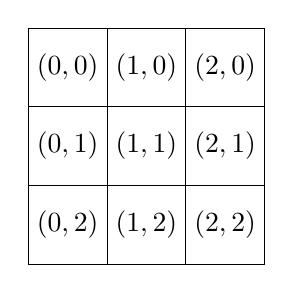
\begin{tikzpicture}
\draw[step=1cm,black,very thin] (0,0) grid (3,3);
\node at (0.5,0.5) {$(0, 2)$};
\node at (1.5,0.5) {$(1, 2)$};
\node at (2.5,0.5) {$(2, 2)$};
\node at (0.5,1.5) {$(0, 1)$};
\node at (1.5,1.5) {$(1, 1)$};
\node at (2.5,1.5) {$(2, 1)$};
\node at (0.5,2.5) {$(0, 0)$};
\node at (1.5,2.5) {$(1, 0)$};
\node at (2.5,2.5) {$(2, 0)$};
\end{tikzpicture}

The \scalainline{Solution.createGame} function, which you need to implement,
takes as input the player who makes the first move, the
value $n$ that specifies the dimensions of the board, and a map from coordinates to \scalainline{Player}s
that indicates where the pieces are.

For example:

\begin{itemize}

  \item In generalized tic-tac-toe, either play may make the first move.
  Therefore, given an empty board:

  
\begin{tikzpicture}
  \draw[step=1cm,black,very thin] (0,0) grid (3,3);
  \end{tikzpicture}

  We can call the function in two ways:

  \begin{scalacode}
  Solution.createGame(O, 3, Map())
  Solution.createGame(X, 3, Map())
  \end{scalacode}

\item This board:

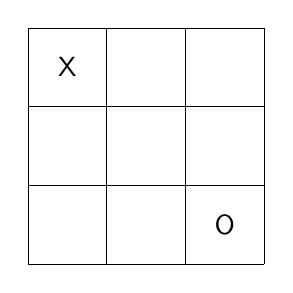
\begin{tikzpicture}
\draw[step=1cm,black,very thin] (0,0) grid (3,3);
\node (a) at (2.5,0.5) {\textsf{O}};
\node (b) at (0.5,2.5) {\textsf{X}};
\end{tikzpicture}

Can be represented as:
\begin{scalacode}
Solution.createGame(X, 3, Map((0, 0) -> X, (2, 2) -> O))
\end{scalacode}
Alternatively, we could have O make the next move.

\item This board:

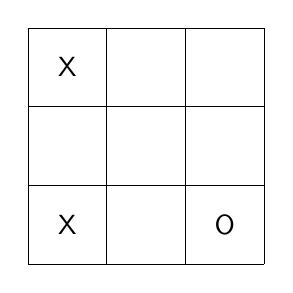
\begin{tikzpicture}
\draw[step=1cm,black,very thin] (0,0) grid (3,3);
\node (a) at (0.5,0.5) {\textsf{X}};
\node (b) at (0.5,2.5) {\textsf{X}};
\node (c) at (2.5,.5) {\textsf{O}};
\end{tikzpicture}

Can be represented as:
\begin{scalacode}
Solution.createGame(X, 3, Map((0, 0) -> X, (0, 2) -> X, (2, 2) -> O))
\end{scalacode}
Alternatively, we could have O make the next move.


\item This board, which is $4 \times 4$:

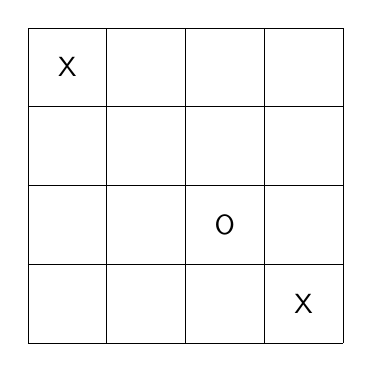
\begin{tikzpicture}
\draw[step=1cm,black,very thin] (0,0) grid (4,4);
\node (a) at (0.5,3.5) {\textsf{X}};
\node (b) at (2.5,1.5) {\textsf{O}};
\node (c) at (3.5, 0.5) {\textsf{X}};
\end{tikzpicture}

Can be represented as:
\begin{scalacode}
Solution.createGame(O, 4, Map((0, 0) -> X, (2, 2) -> O, (3, 3) -> X))
\end{scalacode}
Alternatively, we could have X start first too.

\end{itemize}

\section{The Minimax Algorithm}

\emph{Minimax} is an algorithm to to determine who will win (or draw)
a two-player game, if both players are playing perfectly. To do so, Minimax
searches all possible game-states that are reachable from a given inital
state. Here is an outline of a recursive implementation of Minimax:

\begin{scalacode}
def minimax(game: Game): Some[Player] = {

  /*
  If it is Xs turn:

    1. If X has won the game, return Some(X).
    2. If the game is a draw, return None. (If all squares are filled
       and nobody has won, then the game is a draw. However, you are
       free to detect a draw earlier, if you wish.)
    3. Recursively apply minimax to all the successor states of game
       - If any recursive call produces X, return Some(X)
       - Or, if any recursive call produces None, return None
       - Or, return Some(O)

  The case for Os turn is similar.
  */

}
\end{scalacode}

You can find several other descriptions of Minimax on the Web. But, Minimax
 is a very straightforward function to write, if you follow the programming directions below
and implement (and test) everything leading up to Minimax.

\section{Programming Task}

Your task is to implement a representation of boards, by implementing
the \scalainline{GameLike} trait, provided in the template code.
Your code must be able to implement arbitrary $n \times n$ boards for
all $n > 2$. However, your implementation of the Minimax algorithm
(the \scalainline{MinimaxLike} trait) only needs to be fast enough for
 $n \le 4$.\footnote{If you want to do better, lookup \emph{alpha-beta pruning} on the web.}

I recommend proceeding in the following way, using
\texttt{Solution.scala} as a template:

\begin{enumerate}

\item
   Add fields to the \scalainline{Game} class to represent the state of the game and
   fill in the body of the \scalainline{Solution.createGame(turn, dim, board)} function.
   You may assume that \scalainline{dim >= 2} and that all the pieces described
   in \scalainline{board} are within bounds. However, \emph{The board may be in an
   arbitrary, even illegal state}. For example, the board may have seven Xs.
   Similarly, the \scalainline{turn} could be either X or O.


\item Implement the \scalainline{Game.isFinished} method. Human players often end a game early,
   when the outcome is inevitable. However, you may find it easier to write a
   program that plays until every single square is filled.


\item Implement the \scalainline{getWinner} method.

   \texttt{Provided.scala} has a class called \scalainline{Matrix} that
   has some useful methods. You may find it easier to use a matrix to represent
   a board, instead of an arbitrary map or two-dimensional array.

\item Implement the \scalainline{nextBoards} method, which returns a list of
   boards that represent all the moves the next player could make.

   For example, if the current board looks like this:

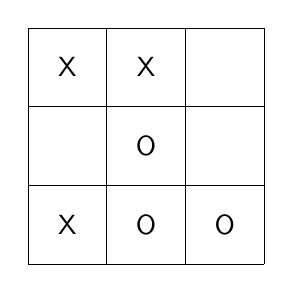
\begin{tikzpicture}
\draw[step=1cm,black,very thin] (0,0) grid (3,3);
\node at (0.5,0.5) {\textsf{X}};
\node at (1.5,0.5) {\textsf{O}};
\node at (2.5,0.5) {\textsf{O}};
\node at (1.5,1.5) {\textsf{O}};
\node at (0.5,2.5) {\textsf{X}};
\node at (1.5,2.5) {\textsf{X}};
\end{tikzpicture}

And if it is \emph{O}'s turn, then these are the three possible next boards:

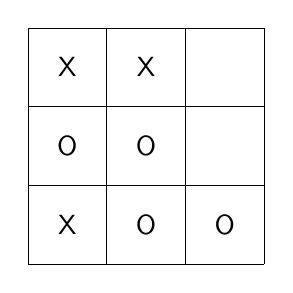
\begin{tikzpicture}
\draw[step=1cm,black,very thin] (0,0) grid (3,3);
\node at (0.5,0.5) {\textsf{X}};
\node at (1.5,0.5) {\textsf{O}};
\node at (2.5,0.5) {\textsf{O}};
\node at (0.5,1.5) {\textsf{O}};
\node at (1.5,1.5) {\textsf{O}};
\node at (0.5,2.5) {\textsf{X}};
\node at (1.5,2.5) {\textsf{X}};
\end{tikzpicture}
\quad
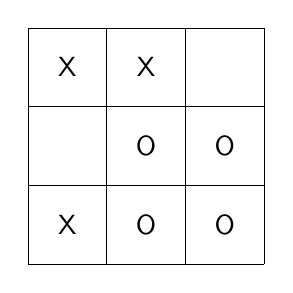
\begin{tikzpicture}
\draw[step=1cm,black,very thin] (0,0) grid (3,3);
\node at (0.5,0.5) {\textsf{X}};
\node at (1.5,0.5) {\textsf{O}};
\node at (2.5,0.5) {\textsf{O}};
\node at (1.5,1.5) {\textsf{O}};
\node at (2.5,1.5) {\textsf{O}};
\node at (0.5,2.5) {\textsf{X}};
\node at (1.5,2.5) {\textsf{X}};
\end{tikzpicture}
\quad
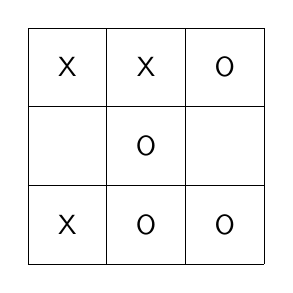
\begin{tikzpicture}
\draw[step=1cm,black,very thin] (0,0) grid (3,3);
\node at (0.5,0.5) {\textsf{X}};
\node at (1.5,0.5) {\textsf{O}};
\node at (2.5,0.5) {\textsf{O}};
\node at (1.5,1.5) {\textsf{O}};
\node at (0.5,2.5) {\textsf{X}};
\node at (1.5,2.5) {\textsf{X}};
\node at (2.5,2.5) {\textsf{O}};
\end{tikzpicture}

\end{enumerate}

As you implement each successive step, you may need to revisit design
decisisions you made earlier.

\section{Hand In}

From \sbt{}, run the command \verb|submit|. The command will create
a file called \verb|submission.tar.gz| in your assignment directory.
Submit this file using Moodle.

For example, if the command runs successfully, you will see output similar
to this:
%
\begin{console}
Created submission.tar.gz. Upload this file to Moodle.
[success] Total time: 0 s, completed Jan 17, 2016 12:55:55 PM
\end{console}

\textbf{Note:}  The command will not allow you to submit code that does not
compile. If your code doesn't compile, you will receive no credit for the
assignment.

\newlecture

\section{Reading}

Programming in Scala, Chapters 12 and 19.

\section{The Singleton Pattern}

\begin{figure}
\begin{javacode}
public class Singleton {
  private static Singleton instance = null;

  private Singleton() { }

  public static Singleton getInstance() {
    if(instance == null) {
      instance = new ClassicSingleton();
    }
    return instance;
  }

  void myMethod() {
    System.out.println("It works")
  }

}
\end{javacode}
\caption{The Singleton Pattern in Java}
\label{javasingleton}
\end{figure}

At times, it is often desirable to only have a single instance of a particular
class. For example, if you have a class that lets you read input from the
user, it doesn't make sense to have two instances, since the user just has
one keyboard. You can create a singleton object in Java by following the
design pattern in \cref{javasingleton}. The only instance of \javainline{Singleton}
that can exist is the one stored in the private field. (Notice that the constructor
is private.) The only way to get
the singleton is by calling the \scalainline{Singleton.getInstance} method.

Here is the equivalent in Scala:

\begin{scalacode}
object Singleton {
  def myMethod() = println("It works")
}
\end{scalacode}

So, all the top-level functions we've created so far (in class and in
assignment) can be thought of as methods of singleton objects.

\section{Case Objects}

We've seen several examples of case classes that take no arguments. For example,
to represent binary trees with values at nodes (and not at the leaves), we could
write the following type:
%
\begin{scalacode}
sealed trait BinTree
case class BinTree(lhs: BinTree, value: Int, rhs: BinTree) extends BinTree
case class Leaf() extends BinTree
\end{scalacode}

However, we can also represent leaves using a \emph{case object}, which is essentially
a singleton that can be used in pattern-matching:
%
\begin{scalacode}
sealed trait BinTree
case class BinTree(lhs: BinTree, value: Int, rhs: BinTree) extends BinTree
case object Leaf extends BinTree
\end{scalacode}

Since \scalainline{Leaf} is an object and not a class, it \emph{cannot}
take any arguments, which why we can simply write \scalainline{Leaf} instead
of \scalainline{Leaf()}. Scala uses case objects extensively. For example,
\scalainline{Nil} and \scalainline{None} are case objects. If they
were case classes, we've have to write \scalainline{Nil()} and
\scalainline{None()} instead.

\section{Subtyping}

Subtyping in Scala is very similar to subtyping in Java.

\begin{notation}
We write $A <: B$ to mean $A$ is a subtype of $B$.
\end{notation}

The intuition behind subtyping is that a subtype always ``adds more features''
to its super-type, and doesn't ``subtract features''. Therefore, if $A <: B$,
then $A$ can be used in any context where $B$ is expected. The context simply
won't try to use the extra features of $A$. However, $B$ \emph{cannot}
be used in contexts where $A$ is expected, because the context may rely on
the ``added features'' of $A$ that $B$ does not provide.

For example, consider the following hierarchy of types, all of which
implement the \scalainline{Animal} trait\footnote{Think of a trait as an interface in Java. Traits
are actually more flexible, but we are only going to use them like interfaces for now.}
%
\begin{scalacode}
trait Animal {
  def sound(): String
}

class Dog extends Animal {
  def sound() = "woof"
  def bite() = "ouch"
}

class Poodle extends Dog {
  override def sound() = "yelp"
}

class Cat extends Animal {
  def sound() = "purr"
  def scratch() = "yow"
}
\end{scalacode}

A function that expects an \scalainline{Animal} can be applied to an object
of any class defined above. Similarly, a function that expects a \scalainline{Dog}
can be applied to a \scalainline{Dog} or a \scalainline{Poodle}, but not to a
\scalainline{Cat}. For example, the following function takes dogs and makes
them bite:
\begin{scalacode}
def dontBite(x: Dog) = {
  x.bite()
}
\end{scalacode}

The expression \scalainline{dontBite(new Cat())} will not type-check, which
is good, because cats don't have a \scalainline{bite} method.

Given the traits and types defined above, we can say that:
\begin{itemize}

  \item \scalainline{Dog <: Animal} because \scalainline{Dog extends Animal}

  \item \scalainline{Poodle <: Dog} because \scalainline{Poodle extends Dog}

  \item \scalainline{Cat <: Animal} because \scalainline{Cat extends Animal}

  \item \scalainline{Poodle <: Animal} because \scalainline{Poodle <: Dog} and
  \scalainline{Dog <: Animal} (subtyping is transitive),

  \item \scalainline{X <: X} for all $X$ (subtyping is reflexive).

\end{itemize}
%
In addition, scala has two special types:
%
\begin{itemize}

  \item \scalainline{X <: Any} for all types X.

  \item \scalainline{Nothing <: X} for all types X.

\end{itemize}

A peculiar property of \scalainline{Nothing} is that
\emph{there are no values with type} \scalainline{Nothing}!
It may seem pointless to have a type with no values. For example, the following
function cannot be applied to anything (not even to \scalainline{null}):
\begin{scalacode}
def useless(x: Nothing): Unit = {
  println("Cannot call me")
}
\end{scalacode}

But, we'll see why \scalainline{Nothing} is useful in a moment.

\section{Generics and Subtyping}

\begin{figure}
\begin{subfigure}[b]{0.26\textwidth}
\begin{scalacode}
def useDog(c: Single[Dog]) = {
  c.get().bite()
}

useDog(new Single(new Cat()))
\end{scalacode}
\caption{Cats can't bite.}
\label{catdog1}
\end{subfigure}
~\vrule~
\begin{subfigure}[b]{0.33\textwidth}
\begin{scalacode}
def useAnimal(c: Single[Animal]) = {
  c.get().sound()
}

val c = new Single[Dog](new Dog())
useAnimal(c)
\end{scalacode}
\label{catdog2}
\caption{Scala is being conservative.}
\end{subfigure}
~\vrule~
\begin{subfigure}[b]{0.31\textwidth}
\begin{scalacode}
def useAnimal2(c: Single[Animal]) = {
  c.set(new Cat())
  c.get().sound()
}

val c = new Single[Dog](new Dog())
useAnimal2(c)
c.get().bite()
\end{scalacode}
\label{catdog3}
\caption{Sneaky function confuses our code.}
\end{subfigure}
\caption{None of these programs type-check.}
\end{figure}

Subtyping becomes more complicated when we working with generics types, such
as lists, sets, or any other kind of container. To illustrate, we'll work
with the following generic type, which is the simplest possible container:
%
\begin{scalacode}
class Container[T](private var x: T) {
  def get(): T = x
  def set(newX: T): Unit = x = newX
}

val c1: Container[Dog] = new Container(new Dog)
c1.set(new Poodle)
\end{scalacode}

Unsurprisingly, we can't store cats in \scalainline{c1}. If we did, a function
that consumes a container with a dog, might try to \scalainline{.get} the
dog and call the \scalainline{bite} method, which cats don't have.
Therefore, the code in \cref{catdog1} does not type-check.
However, since \scalainline{Dog <: Animal}, can we send a dog-container
to a function that expects an animal container. For example, \cref{catdog2}
appears to be safe. Unfortunately, this code does not type-check either. Although this particular example
is safe, consider the variation in \cref{catdog3}.

The problem above is that \scalainline{useAnimal2} sneakily stores a cat in
the container. After the function returns, \scalainline{c.get} would produce
a cat even though the type indicates that it should produce a dog.
Therefore, the Scala type-checker does not allow this program to type-check.

Unfortunately, \cref{catdog2} (which was safe) does not type-check either, just so that
this kind of unsafe example can be ruled out. Individual methods and functions
are type-checked only once. Similarly, when a function or method call is type-checked,
the body of the function is not re-examined.

\section{Variance}

However, lists and other immutable data structures in Scala are not constrained
this way. For example, the following code does type-check:

\begin{scalacode}
def useAnimals(alist: List[Animal]) = {
  alist.map(animal => animal.sound()).mkString(", ")
}

val lst: List[Cat] = List(new Cat(), new Cat())
useAnimals(lst)
\end{scalacode}

The reason this works is because there are no methods on lists to update
their contents. The problem with our \scalainline{Container[T]} class is
that it writes to \scalainline{T}-typed values. However, if we had a functional
container class, we can use a \emph{covariance annotation} to indicate
that \scalainline{T}-typed values are never updated.

\begin{scalacode}
class Container[+T](private val x: T) {
  def get(): T = x
}
\end{scalacode}

The \scalainline{+T} annotation indicates \scalainline{Container[A] <:
Container[B]} when \scalainline{A <: B}. For this to be safe,
Scala ensures that \scalainline{T}-typed values are never updated
by the class.\footnote{Coavariance is actually more subtle than this. The reading discusses it in more depth, but you don't have to remember all the details.} (The class may have other kind of state, but it can't
update \scalainline{T}s.)

As a rule of thumb, almost any immutable data structure can be made
covariant, which makes it more flexible. E.g., we can a \scalainline{Set[Cat]}
where a \scalainline{Set[Animal]} is expected or a \scalainline{List[Dog]}
where a \scalainline{List[Animal]} is expected.

In fact, the list type in Scala is covariant:
%
\begin{scalacode}
sealed trait List[+A]
\end{scalacode}
Cons is easy to define as follows:
\begin{scalacode}
case class ::[A](head: A, tail: List[A]) extends List[A]
\end{scalacode}
However, the definition of \scalainline{Nil} is trickier. If it were a case-class,
we could write:
\begin{scalacode}
case class Nil[A]() extends List[A]
\end{scalacode}
However, recall that \scalainline{Nil} is a case-object. So, we may try to
write this:
\begin{scalacode}
case object Nil[A] extends List[A]
\end{scalacode}
However, objects can't have type parameters (or any parameters for that matter).

As discussed earlier, Scala has a special type \scalainline{Nothing} that has no values
and is the subtype of all other types: i.e.,
\scalainline{Nothing <: A}. Therefore, by covariance of lists, \scalainline{List[Nil] <: List[A]}, so
we can write:
\begin{scalacode}
case object Nil extends List[Nothing]
\end{scalacode}
Although there a no values of type \scalainline{Nothing}, an empty list of
of type \scalainline{List[A]} doesn't contain any values of type \scalainline{A}.
Therefore, the \scalainline{Nil} object can be given the type \scalainline{List[Nothing]}.

\newdiscussion{TODO -- ??? (Feb 24)}

\newlecture


\section{Bounded Quantification}

\begin{figure}
\begin{scalacode}
def insert[A](toInt: A => Int, x: A, alist: List[A]): List[A] = alist match {
  case hd :: tl => if (toInt(x) <= toInt(hd)) { x :: hd :: tl } else { hd :: insert(toInt, x tl) }
  case Nil => List(x)
}

def sort[A](toInt: A => Int, alist: List[A]): List[A] = alist match {
  case Nil => Nil
  case hd :: tl => insert(toInt, hd, sort(toInt, tl))
}
\end{scalacode}
\caption{Sorting by mapping values to integers.}
\label{sortToIntHOF}
\end{figure}

We've used higher-order functions to write generic sorting functions.
\Cref{sortToIntHOF} is small variation of the kind of function we've
seen before: instead of taking a comparator function as an argument, it takes a
\scalainline{toInt} function that maps
\scalainline{A}-values to integers, then sorts by the natural ordering
on integers.

For example, given this type:
\begin{scalacode}
case class Person(name: String, age: Int)
\end{scalacode}
We can sort people in ascending order by age:
\begin{scalacode}
val personList: List[Person] = ...
sort((p: Person) => p.age, personList)
\end{scalacode}

However, it can be annoying to pass the \scalainline{toInt} function around,
especially since there is a natural ordering for \scalainline{Person}s.
We can address this issue by adding a \scalainline{toInt} method
to \scalainline{Person} and modifying \scalainline{insert} to invoke this
method instead:
\begin{scalacode}
def insert[A](x: A, alist: List[A]): List[A] = alist match {
  case hd :: tl => if (x.toInt <= hd.toInt) ...
  case Nil => ...
}
\end{scalacode}
Unfortunately, this code does not type-check: \scalainline{x} and \scalainline{hd} both have type \scalainline{A},
would could be \emph{any} type. There is no guarantee that \scalainline{A}-values have a \scalainline{toInt}
method.

\begin{figure}
\begin{scalacode}
trait IntLike {
  def toInt(): Int
}

case class Person(name: String, age: Int) extends IntLike {
  def toInt(): Int = age
}

def insert(x: IntLike, alist: List[IntLike]): List[IntLike] = alist match {
  case Nil => List(x)
  case hd :: tl => if (x.toInt <= hd.toInt) { x :: hd :: tl } else { hd :: insert(x, tl) }
}

def sort(alist: List[IntLike]): List[IntLike] = alist match {
  case Nil => Nil
  case hd :: tl => insert(hd, sort(tl))
}
\end{scalacode}
\caption{This code type-checks, but the types lose too much information.}
\label{sorting_fail}
\end{figure}

We can address this problem by introducing a trait for objects that have a
\scalainline{ToInt} method and modify \scalainline{Person} to extend this trait.
We could then rewrite the sorting function, as shown in \cref{sorting_fail}.
Unfortunately, the type of \scalainline{sort} is not helpful. When we apply
it to a \scalainline{List[Person]}, we get back a list \scalainline{List[IntLike]},
and loose track of the fact that we were working with \scalainline{Person}s:
\begin{scalacode}
val alist = List(Person("Alice", 12), Person("Bob", 7), Person("Carol", 3))
val sortedList = sort(alist)
sortedList.head.age // type error, since head has type IntLike
\end{scalacode}

We need to know that the type of the argument and the type of the result
of \scalainline{sort} are the same, which is what generics did for us:
%
\begin{scalacode}
def sort[A](alist: List[A]): List[A]
\end{scalacode}
However, the problem with this generic type was that \scalainline{A} could
be any type, and not necessary a type with a \scalainline{toInt} method,
which is what this type ensured:
\begin{scalacode}
def sort(alist: List[IntLike]): List[IntLike]
\end{scalacode}
We need to
ensure that \scalainline{alist} and the result have the same type \emph{and}
that they implement \scalainline{IntLike}. We can do this by using
\emph{bounded quantification}:
\begin{scalacode}
def sort[A <: IntLike](alist: List[A]): List[A]
\end{scalacode}
You should read this as ``sort consumes and produces lists of $A$, where $A$
is a subtype of IntLike''. \Cref{sort_bq} shows a complete version of this code.
Note that none of this is Scala-specific. \Cref{sorting_java_omg} converts
this code into Java.

Finally, note that when we write:
\begin{scalacode}
def sort[A](alist: List[A]): List[A]
\end{scalacode}
What we're really saying is that \scalainline{A} can be any type, or:
%
\begin{scalacode}
def sort[A <: Any](alist: List[A]): List[A]
\end{scalacode}
%
The bound \scalainline{Any} is implicit. Using bounded quantification, we're restricting \scalainline{A} to be any
type that implements \scalainline{IntLike}.

\begin{figure}
\begin{scalacode}
def insert[A <: IntLike](x: A, alist: List[A]): List[A] = alist match {
  case Nil => List(x)
  case hd :: tl => if (x.toInt <= hd.toInt) { x :: hd :: tl } else { hd :: insert(x, tl) }
}

def sort[A <: IntLike](alist: List[A]): List[A] = alist match {
  case Nil => Nil
  case hd :: tl => insert(hd, sort(tl))
}
\end{scalacode}
\caption{A well-typed sort using bounded quantification.}
\label{sort_bq}
\end{figure}

\begin{figure}
\begin{javacode}
interface IntLike {
  int toInt();
}

class Person implements IntLike {
  String name;
  int age;
  Person(String name, int age) { this.name = name; this.age = age; }
  public int toInt() { return age; }
}

interface List<T>  { }
class Empty<T> implements List<T> { }
class Cons<T> implements List<T> {
  public final T head;
  public final List<T> tail;
  public Cons(T head, List<T> tail) {
    this.head = head;
    this.tail = tail;
  }
}

class Sorting {

  static <T extends IntLike> List<T> insert(T x, List<T> alist) {
    if (alist instanceof Empty) {
      return new Cons<T>(x, new Empty<T>());
    }
    else {
      T hd = ((Cons<T>)alist).head;
      List<T> tl = ((Cons<T>)alist).tail;
      if (x.toInt() < hd.toInt()) {
        return new Cons<T>(x, new Cons<T>(hd, tl));
      }
      else {
        return new Cons<T>(hd, insert(x, tl));
      }
    }
  }

  static <T extends IntLike> List<T> sort(List<T> alist) {
    if (alist instanceof Empty) {
      return alist;
    }
    else {
      T hd = ((Cons<T>)alist).head;
      List<T> tl = ((Cons<T>)alist).tail;
      return insert(hd, sort(tl));
    }
  }

}
\end{javacode}
\caption{\Cref{sort_bq} converted into Java (with lists and person too).}
\label{sorting_java_omg}
\end{figure}

\section{Type Parameters to Traits}

Traits in Scala (and interfaces in Java) can take type arguments.
For example, the following trait T takes three type arguments:
\begin{scalacode}
trait T[X,Y,Z] {
  def f(x: X): Y
  def g(z: Z): Z
}
\end{scalacode}
Therefore, when a class extends the trait, it needs to supply type-arguments:
\begin{scalacode}
class C1 extends T[???, ???, ???] {
  def f(x: Int): String = x.toString
  def g(z: Boolean): Boolean = !z
}
\end{scalacode}
We can infer the arguments by examining the body of the
class.\footnote{Surprisingly, Scala's type-inference cannot infer these arguments for us.}
\begin{itemize}
  \item The class states that the argument of \scalainline{f} is an \scalainline{Int}
  and the trait states that the argument of \scalainline{f} is an \scalainline{X}.
  Therefore, \scalainline{X = Int}.

  \item The class states that the result of \scalainline{f} is a \scalainline{String}
  and the trait states that the result of \scalainline{f} is a \scalainline{Y}.
  Therefore, \scalainline{Y = String}.

  \item The class states that the argument and result of \scalainline{g} are both \scalainline{Boolean}
  and the trait states that the argument and result of \scalainline{g} are both \scalainline{Z}.
  Therefore, \scalainline{Z = Int}.
\end{itemize}
Therefore, the class can extend the trait as follows:
\begin{scalacode}
class C1 extends T[Int, String, Boolean] {
  def f(x: Int): String = x.toString
  def g(z: Boolean): Boolean = !z
}
\end{scalacode}

Consider the following class that is trying to extend the same trait:
\begin{scalacode}
class C2 extends T[Int, String, ???] {
  def f(x: Int): String = x.toString
  def g(z: Boolean): Int = 42
}
\end{scalacode}
This extension is impossible, since it would imply that \scalainline{Boolean = Int}, which
is a contradiction.

Consider the following class:
\begin{scalacode}
class C3(head: Int, tail: C3) extends T[???, ???, ???] {
  def f(x: Int): C3 = new C3(x, this)
  def g(z: C3): C3 = z
}
\end{scalacode}
We can reason through the type parameters in exactly the same way as before:
\begin{itemize}
  \item The class states that the argument of \scalainline{f} is an \scalainline{Int}
  and the trait states that the argument of \scalainline{f} is an \scalainline{X}.
  Therefore, \scalainline{X = Int}.

  \item The class states that the result of \scalainline{f} is a \scalainline{C3}
  and the trait states that the result of \scalainline{f} is a \scalainline{Y}.
  Therefore, \scalainline{Y = C3}.

  \item The class states that the argument and result of \scalainline{g} are both \scalainline{C3}
  and the trait states that the argument and result of \scalainline{g} are both \scalainline{Z}.
  Therefore, \scalainline{Z = C3}.
\end{itemize}
Here is the complete definition:
\begin{scalacode}
class C3(head: Int, tail: C3) extends T[Int, C3, C3] {
  def f(x: Int): C3 = new C3(x, this)
  def g(z: C3): C3 = z
}
\end{scalacode}

Consider the following generalization:
\begin{scalacode}
class C4[A](head: A, tail: C4[A]) extends T[???, ???, ???] {
  def f(x: A): C4[A] = new C4[A](x, this)
  def g(z: C4[A]): C4[A] = z
}
\end{scalacode}

We can apply the same reasoning to get:
\begin{scalacode}
class C4[A](head: A, tail: C4[A]) extends T[Int, C4[A], C4[A]] { ... }
\end{scalacode}

\begin{instructor}
Note that we have not covered covariant/contravariant type-arguments to traits.
\end{instructor}

\section{Leveraging Recursive Bounded Quantification}

It is cumbersome to sort values by explicitly mapping them to integers,
which is what we did before.
E.g., if we wanted to people sort by name, it would be very annoying to convert
all names to unique integers. Alternative, if we want to sort a list of time
objects, it would be annoying (and needless) to convert them all to seconds
from some fixed date.\footnote{Most computers store the current time as the number of seconds elapsed since Jan 1, 1970.}

A better approach would be to give sortable classes a \scalainline{lessThan} method
and then have them inherit from a common trait:
\begin{scalacode}
case class Person(name: String, age: Int) extends Comparable = {
  def lessThan(other: Person): Boolean = this.name < other.name
}
case class Time(h: Int, m: Int, s: Int) extends Comparable = {
  def lessThan(o: Time): Boolean = this.h < o.h || (this.h == o.h && this.m < o.min || (this.m == o.min && this.s < o.s))
}
\end{scalacode}
But, defining \scalainline{Comparable} is tricky:
\begin{scalacode}
trait Comparable {
  def lessThan(other: ???): Boolean
}
\end{scalacode}
The problem is that \scalainline{Person} requires the type of the argument
to be \scalainline{Person}, whereas \scalainline{Time} requires it to be \scalainline{Time}.
However, \scalainline{Comparable} should be a generic trait that any type can extend.
When a type in a trait must vary, we can simply turn it into a type variable,
\begin{scalacode}
trait Comparable[T] {
  def lessThan(other: T): Boolean
}
\end{scalacode}
However, the definitions of \scalainline{Person} and \scalainline{Time}
above are now incomplete, since they extend \scalainline{Comparable}, which
takes a type argument:
\begin{scalacode}
case class Person(name: String, age: Int) extends Comparable[???] = {
  def lessThan(other: Person): Boolean = ...
}
case class Time(h: Int, m: Int, s: Int) extends Comparable[???] = {
  def lessThan(o: Time): Boolean = ...
}
\end{scalacode}
We can reason about the types in exactly the way we did before.
For example, \scalainline{Person} states that the argument of \scalainline{lessThan}
is \scalainline{Person}, whereas the trait states that it is \scalainline{T}.
Therefore, \scalainline{T = Person}:
\begin{scalacode}
case class Person(name: String, age: Int) extends Comparable[Person] = ...
\end{scalacode}
We can make a similar argument for \scalainline{Time}:
\begin{scalacode}
case class Time(h: Int, m: Int, s: Int) extends ComparableTime = ...
\end{scalacode}

Now that both classes extend the \scalainline{Comparable[T]} trait, let's
update \scalainline{insert} to use it. Here is our first attempt, which
uses generics to constrain the type of the argument and result:
%
\begin{scalacode}
def insert[A](x: A, alist: List[A]): List[A] = alist match {
  case Nil => List(x)
  case head :: tail => if (x.lessThan(head)) { x :: head :: tail } else { head :: insert(x, tail) }
}
\end{scalacode}
As before, this code will not type-check, since \scalainline{A} could be any
type, whereas the body requires \scalainline{A}-typed objects to have a \scalainline{lessThan}
method. Fortunately, we have a trait for these kinds of objects:
\begin{scalacode}
def insert[A <: Comparable](x: A, alist: List[A]): List[A] = ...
\end{scalacode}
However, this will not type-check either, because \scalainline{Comparable} needs
a type argument. So, we really need to write something like this:
\begin{scalacode}
def insert[A <: Comparable[???]](x: A, alist: List[A]): List[A] = ...
\end{scalacode}

Let's reason through this systematically again:
%
\begin{itemize}

  \item \scalainline{x} has type $\scalainline{A <: Comparable[???]}$,

  \item \scalainline{x.lessThan} takes an argument of type \scalainline{???},

  \item \scalainline{x.lessThan} is applied to \scalainline{head}, which has
  type \scalainline{A},

  \item Therefore, \scalainline{??? = A}.

\end{itemize}

\Cref{sort_sortable_complete} shows a complete version of sorting using
the \scalainline{Comparable} trait.

\begin{figure}
\begin{scalacode}
trait Comparable[T] {
  def lessThan(other: T): Boolean
}

def insert[A <: Comparable[A]](x: A, alist: List[A]): List[A] = alist match {
  case Nil => List(x)
  case head :: tail => if (x.lessThan(head)) { x :: head :: tail } else { head :: insert(x, tail) }
}

def sort[A <: Comparable[A]](alist: List[A]): List[A] = alist match {
  case Nil => Nil
  case head :: tail => insert(x, sort(tail))
}
\end{scalacode}
\caption{Sorting with a recursive bound.}
\label{sort_sortable_complete}
\end{figure}

\section{Expression Evaluator}


\begin{figure}
\begin{minipage}{0.45\textwidth}
\begin{scalacode}
sealed trait Expr
case class Const(n: Int) extends Expr
case class Add(e1: Expr, e2: Expr) extends Expr
case class Mul(e1: Expr, e2: Expr) extends Expr
case class Sub(e1: Expr, e2: Expr) extends Expr
case class Div(e1: Expr, e2: Expr) extends Expr

def eval(expr: Expr): Int = expr match {
  case Const(n) => n
  case Add(e1, e2) => eval(e1) + eval(e2)
  case Mul(e1, e2) => eval(e1) * eval(e2)
  case Sub(e1, e2) => eval(e1) - eval(e2)
  case Div(e1, e2) => eval(e1) / eval(e2)
}
\end{scalacode}
\caption{Evaluation with \scalainline{Int}s.}
\label{intEval}
\end{minipage}
\quad\vrule\quad
\begin{minipage}{0.45\textwidth}
\begin{scalacode}
sealed trait Expr
case class Const(n: Float) extends Expr
case class Add(e1: Expr, e2: Expr) extends Expr
case class Mul(e1: Expr, e2: Expr) extends Expr
case class Sub(e1: Expr, e2: Expr) extends Expr
case class Div(e1: Expr, e2: Expr) extends Expr

def eval(expr: Expr): Float = expr match {
  case Const(n) => n
  case Add(e1, e2) => eval(e1) + eval(e2)
  case Mul(e1, e2) => eval(e1) * eval(e2)
  case Sub(e1, e2) => eval(e1) - eval(e2)
  case Div(e1, e2) => eval(e1) / eval(e2)
}
\end{scalacode}
\caption{Evaluation with \scalainline{Double}s.}
\label{doubleEval}
\end{minipage}
\caption{Two very similar evaluators.}\label{twoevals}
\end{figure}


We've seen that we can use case-classes to represent arithmetic expressions
and how to write a simple, recursive evaluator. Consider the two evaluators
in \cref{twoevals}. The only difference between them is that \cref{intEval}
evaluators integer-valued expressions whereas \cref{doubleEval} evaluates
float-valued expressions. We should be able to abstract away their commonalities
by creating a generic type:

\begin{scalacode}
sealed trait Expr[A]
case class Const[A](n: A) extends Expr[A]
case class Add[A](e1: Expr[A], e2: Expr[A]) extends Expr[A]
case class Mul[A](e1: Expr[A], e2: Expr[A]) extends Expr[A]
case class Sub[A](e1: Expr[A], e2: Expr[A]) extends Expr[A]
case class Div[A](e1: Expr[A], e2: Expr[A]) extends Expr[A]
\end{scalacode}

With this type, we can write integer-valued expressions:
\begin{scalacode}
val e1: Expr[Int] = Add(Const(12), Const(3))
\end{scalacode}
and float-valued expressions too:
\begin{scalacode}
val e1: Expr[Double] = Div(Const(12), Const(5))
\end{scalacode}

The obvious way to generalize \scalainline{eval} is as follows:

\begin{scalacode}
def eval[A](expr: Expr[A]): A = expr match {
  case Const(n) => n
  case Add(e1, e2) => eval(e1) + eval(e2)
  ...
}
\end{scalacode}

Unfortunately, this doesn't work. The problem is that \scalainline{eval(e1)}
and \scalainline{eval(e2)} produce values of type \scalainline{A}, which could
be \emph{any} type. There is no guarantee that values of this type can
be added, multiplied, and so on. For example, we could have written:

\begin{scalacode}
val e1: Expr[String] = Div(Const("Hello"), Const("Goodbye"))
\end{scalacode}

The problem is that the type of \scalainline{eval} is too generic: it should
only be applicable to a type with addition, division, etc. defined appropriately.
We can define a trait that defines these operations:

\begin{scalacode}
trait NumLike[A] {
  def add(other: A): A
  def mul(other: A): A
  def sub(other: A): A
  def div(other: A): A
}
\end{scalacode}

We can create a wrapper for \scalainline{Int} and \scalainline{Double}
that implements this trait:

\begin{scalacode}
case class N(n: Int) extends NumLike[N] {
  def add(other: N): N = N(n + other.n)
  def mul(other: N): N = N(n * other.n)
  def sub(other: N): N = N(n - other.n)
  def div(other: N): N = N(n / other.n)
}

case class F(x: Double) extends NumLike[F] {
  def add(other: F): N = F(f + other.f)
  def mul(other: F): N = F(f * other.f)
  def sub(other: F): N = F(f - other.f)
  def div(other: F): N = F(f / other.f)
}
\end{scalacode}

We can now define the evaluator as follows:

\begin{scalacode}
def eval[T <: NumLike[T]](expr: Expr[T]): T = expr match {
  case Const(n) => n
  case Add(e1, e2) => eval(e1).add(eval(e2))
  case Mul(e1, e2) => eval(e1).mul(eval(e2))
  case Sub(e1, e2) => eval(e1).sub(eval(e2))
  case Div(e1, e2) => eval(e1).div(eval(e2))
}
\end{scalacode}

Although we've managed to reuse a lot of code in our evaluator,
we had to wrap \scalainline{Int}s and \scalainline{Double}s, which was
quite annoying. We'll learn how to address this problem soon.

\section{Bounded Quantification in the Java and Scala standard libraries}

Bounded quantification is used extensively in libraries. For example,
here is the signature of the \javacode{Integer} class in Java:

\begin{scalacode}
public final class Integer extends Number implements Comparable<Integer>
\end{scalacode}

The standard \javacode{Comparable} interface is very similar to the one we
defined.


\newhw{Generics}

\newlecture

\section{The \emph{Same Fringe} Problem}

\begin{figure}
\begin{scalacode}
def fringe[A](t: BinTree[A]): List[A] = t match {
  case Leaf(x) => List(x)
  case Node(lhs, rhs) => fringe(lhs) ++ fringe(rhs)
}
\end{scalacode}
\caption{Recursively calculating the fringe of a binary tree.}
\label{fringeRec}
\end{figure}

Given a binary tree:

\begin{scalacode}
sealed trait BinTree[+A]
case class Node[A](lhs: BinTree[A], rhs: BinTree[A]) extends BinTree[A]
case class Leaf[A](x: A) extends BinTree[A]
\end{scalacode}

The \emph{fringe} of a binary tree are the values in left-to-right order. For
example, the fringe of the following tree:
\begin{scalacode}
val t1 = Node(Leaf(10), Node(Leaf(20), Leaf(40)))
\end{scalacode}
is $10$, $20$, and $40$, in that order. The \emph{same-fringe problem} is to write
a function to determine if two trees have the same fringe. For
example the following tree:
%
\begin{scalacode}
val t2 = Node(Node(Leaf(10), Leaf(20)), Leaf(40))
\end{scalacode}
Has the same fringe as \scalainline{t1}.

We can write a simple recursive function to calculate the fringe of a tree,
as shown in \cref{fringeRec}, so a simple solution to the same-fringe problem
is:
\begin{scalacode}
fringe(t1) == fringe(t2)
\end{scalacode}

But, this is not a very efficient solution:
\begin{itemize}

  \item If the trees are very large, we'll spend a lot of time appending
  lists, and

  \item If the fringes are different, we'll generate the entire fringe instead
  of terminating as soon as a difference is detected.

\end{itemize}

\section{An Imperative Solution}

\begin{figure}
\begin{scalacode}
class FringeIterator[A](tree: BinTree[A]) extends Iterator[A] {
  private val stack = collection.mutable.Stack(tree)
  def hasNext = stack.isEmpty
  def next() = {
    val top = stack.pop()
    top match {
      case Leaf(x) => x
      case Node(lhs, rhs) => { stack.push(rhs); stack.push(lhs); next() }
    }
  }
}

def sameFringe[A](t1: BinTree[A], t2: BinTree[A]): Boolean = {
  val iter1 = new FringeIterator(t1)
  val iter2 = new FringeIterator(t2)
  while (iter1.hasNext && iter2.hasNext) {
    val x = iter1.next
    val y = iter2.next
    if (x != y) {
      return false
    }
  }
  return !iter1.hasNext && !iter2.hasNext
}
\end{scalacode}
\caption{An imperative solution.}
\label{samefringe_imperative}
\end{figure}

- Describe the imperative solution
- Seems to be fundamentally imperative: each call to .next returns a new value,
  which means that iter1 must use mutable state internally
- Consider writing list-equal for for JoinLists: very similar, but trickier
  iterator


\section{A Functional Solution}

\begin{figure}
\begin{scalacode}
class Generator[T](val gen: () => Option[(T, Generator[T])]) { self =>
  def andThen(rest: () => Generator[T]): Generator[T] = new Generator[T](() => self.gen() match {
      case None => rest().gen()
      case Some((x, lhsRest)) => Some((x, lhsRest.andThen(rest)))
  })
}

object Generator {
  def one[T](x: T) = new Generator[T](() => Some((x, new Generator[T](() => None))))
}

def fringe[T](t: BinTree[T]): Generator[T] = t match {
  case Leaf(x) => Generator.one(x)
  case Node(lhs, rhs) => fringe(lhs).andThen(() => fringe(rhs))
}

def sameFringeRec[T](t1: Generator[T], t2: Generator[T]): Boolean = (t1.gen(), t2.gen()) match {
  case (None, None) => true
  case (Some((x, t1Rest)), Some((y, t2Rest))) => x == y && sameFringeRec(t1Rest, t2Rest)
  case _ => false
}

def sameFringe[T](t1: BinTree[T], t2: BinTree[T]) = sameFringeRec(fringe(t1), fringe(t2))
\end{scalacode}
\caption{A functional solution.}
\label{sameFringeFun}
\end{figure}


\newdiscussion{TODO -- Dan (Mar 2)}

\newlecture

\newhw{Kitchen Sink: Pre-Spring Break Assignment}

Something that covers everything, due after Spring Break. Try to make students
write at least 700 lines of code.

\newlecture

\newlecture

\section{Type members}

You've already learned how to write a \emph{Reverse Polish Notation} calculator
in 187. In this lecture, we'll talk about \emph{Polish Notation}.

We'll use the following type definition to represent individual instructions:
%
\begin{scalacode}
sealed trait Instr
case class IInt(n: Int) extends Instr
case object IAdd extends Instr
case object IMul extends Instr
case object ISub extends Instr
\end{scalacode}


The RPN calculator you wrote in 187 could be written using an imeperative stack
in Scala, as shown in \cref{rpnImperative}. But, a cleaner and shorter
implementation using recursion and pattern matching is shown in \cref{rpnCalc}.

\begin{think}
The functional calculator calls \scalainline{sys.error} to explicitly throw
errors, but the imperative version does not. How do errors occur in the
imperative version? Do you see the bug in the code?
\end{think}

\begin{figure}
\begin{minipage}{0.45\textwidth}
\begin{scalacode}
def rpnCalc(instructions: List[Instr]) {
  val stack = collection.mutable.Stack[Int]()

  var instrs = instructions
  while (instrs.isEmpty == false) {
    val instr = instrs.head
    instrs = instrs.tail
    instr match {
      case IInt(n) => stack.push(n)
      case IAdd => {
        val n2 = stack.pop()
        val n1 = stack.pop()
        stack.push(n1 + n2)
      }
      case IMul => {
        val n2 = stack.pop()
        val n1 = stack.pop()
        stack.push(n1 * n2)
      }
      case ISub => {
        val n2 = stack.pop()
        val n1 = stack.pop()
        stack.push(n1 - n2)
      }
    }
  }

  stack.pop()
}
\end{scalacode}
\caption{An imperative RPN calculator}.
\end{minipage}
\quad
\vrule
\quad
\begin{minipage}{0.45\textwidth}
\begin{scalacode}
def doRpn(e: List[Instr], stack: List[Int]): List[Int] =
  (e, stack) match {
    case (Nil, stack) => stack
    case (IInt(n) :: rest, stack) => doRpn(rest, n :: stack)
    case (IAdd :: rest, n2 :: n1 :: stack) =>
      doRpn(rest, (n1 + n2) :: stack)
    case (IMul :: rest, n2 :: n1 :: stack) =>
      doRpn(rest, (n1 * n2) :: stack)
    case (ISub :: rest, n2 :: n1 :: stack) =>
      doRpn(rest, (n1 - n2) :: stack)
    case _ => sys.error("ill-formed expression")
  }

def rpnCalc(instructions: List[Instr]) =
  doRpn(instructions, Nil) match {
    case List(n) => n
    case _ => sys.error("ill-formed expression")
  }
\end{scalacode}
\caption{A functional RPN calculator.}
\label{rpnCalc}
\end{minipage}
\caption{Two RPN Calculators}
\end{figure}


In Polish Notation, as opposed to Reverse Polish Notation, we write the operator
before its operands. Therefore, instead of writing \texttt{1 2 +}, we'll write
\texttt{+ 1 2}. Similarly, instead of writing \texttt{1 3 4 - +}, we'll write
\texttt{+ 1 - 3 4}. Notice that this example shows that you can't simply reverse
the list and use an RPN calculator to evaluate a PN expression.

How should we write a PN calculator? It is important to realize that it
\emph{cannot be written with a loop}. We can try to setup the solution in the
same way as the imperative \scalainline{rpnCalc}, but we'd get stuck in the
cases for the instructions. The problem is that when we see an instruction
such as \scalainline{IAdd}, its operands are not yet on the stack.
In the simplest case, we need to evaluate the next two instructions, e.g.,
in \scalainline{List(IAdd, IInt(2), IInt(3))}. However, there may
be nested expression:
\begin{scalacode}
List(IAdd, IInt(2), ISub, IInt(10), IInt(20))
\end{scalacode}
And there may be instructions for the context. E.g., the following list
of instructions is valid, so long as it's the tail of a list that has
some other operand as its head:
\begin{scalacode}
List(IAdd, IInt(2), IInt(2), IInt(20))
\end{scalacode}




\begin{instructor}
This lecture uses imperative code. Don't use the course plugin. But, setup
\texttt{build.sbt}:

\begin{scalacode}
scalaVersion := "2.11.7"
libraryDependencies += "org.scalatest" %% "scalatest" % "2.2.6" % "test"
\end{scalacode}
\end{instructor}

In this lecture, we'll talk about functions that make lots of recursive calls.
As you know, recursive functions seem to use the stack, so deeply recursive
functions can actually run out of stack space and throw a
\scalainline{StackOverflowError}.

The usual definition of factorial is a simple example of this problem:
\begin{scalacode}
def fac(n: Int): Int = if (n == 0) 1 else (n * fac(n - 1))
\end{scalacode}

If your input is large enough, say \scalainline{fac(5000000)}, the program
will throw a \scalainline{StackOverflowError} on most systems.
You can adjust the size of the stack to make it larger (or smaller), but there
is always an upper-bound.\footnote{For example, use \texttt{java -Xss5m} to
use a 5MB stack. You can pass JVM options into SBT by prefixing them with \texttt{-J}. E.g., \texttt{sbt -J-Xss5m}.}







\newdiscussion{TODO -- Dan (Mar 9)}

\newlecture

\chapter{Homework 8: Tic Tac Toe}

\newlecture

\newdiscussion{TODO -- ??? (Mar 23)}

\newlecture

\newlecture

\newdiscussion{TODO -- Dan (Mar 30)}

\chapter{Homework 9: Sudoku}

\newlecture

\newlecture

\newdiscussion{TODO -- ??? (Apr 6)}

\chapter{Homework 10: Parsing}

\newlecture

\newlecture

\newdiscussion{TODO -- Dan (Apr 13)}

\chapter{Homework 11: ??}

\newlecture

\newlecture

\chapter{Homework 12: ??}

\newlecture

\newlecture

\newdiscussion{TODO -- Dan (Apr 27)}



\end{document}